\documentclass{article}
\usepackage{titlesec}

\usepackage[citestyle=authortitle-terse,backref,backend=bibtex]{biblatex}
\addbibresource{homotopy-theory.bib}

\setcounter{secnumdepth}{0}
\usepackage{sectsty}
\sectionfont{\fontsize{13}{20}\selectfont}

\usepackage[left=4cm, right=4cm]{geometry}
\usepackage{palatino,eulervm,dutchcal,xcolor}%fonts
\usepackage{graphicx,subcaption,float}
\usepackage{enumitem,parskip,multicol,array}
\newcolumntype{L}{>{$}c<{$}}%table in mathmode
\usepackage{amsthm,amssymb,amsmath,mathtools,thmtools}
\usepackage{tikz,tikz-cd}
\usetikzlibrary{%
	matrix,%
	calc,%
	arrows,%
	shapes,
	decorations.markings,backgrounds,calc,intersections}
\tikzcdset{scale cd/.style={every label/.append style={scale=#1},
		cells={nodes={scale=#1}}}}
\usepackage[bookmarks,bookmarksopen,bookmarksdepth=3]{hyperref}
\hypersetup{%colores
	colorlinks=true,
	urlcolor=blue,
	linkcolor=magenta,
	citecolor=blue,
	filecolor=blue,
	urlbordercolor=white,
	linkbordercolor=white,
	citebordercolor=white,
	filebordercolor=white}
\usepackage{cleveref}

\setcounter{secnumdepth}{0}
\usepackage{sectsty}
\sectionfont{\fontsize{13}{20}\selectfont}

\definecolor{blue-violet}{rgb}{0.54, 0.17, 0.89}
\definecolor{azure}{rgb}{0.0, 0.5, 1.0}
\definecolor{green(ncs)}{rgb}{0.0, 0.62, 0.42}
\definecolor{forestgreen}{rgb}{0.13, 0.55, 0.13}
\definecolor{limegreen}{rgb}{0.2, 0.8, 0.2}
\definecolor{palatinateblue}{rgb}{0.15, 0.23, 0.89}
\definecolor{trueblue}{rgb}{0.0, 0.45, 0.81}
\definecolor{goldenyellow}{rgb}{1.0, 0.87, 0.0}
\definecolor{fashionfuchsia}{rgb}{0.96, 0.0, 0.63}
\definecolor{brightcerulean}{rgb}{0.11, 0.67, 0.84}
\definecolor{jonquil}{rgb}{0.98, 0.85, 0.37}
\definecolor{lavendermagenta}{rgb}{0.93, 0.51, 0.93}
\definecolor{peru}{rgb}{0.8, 0.52, 0.25}
\definecolor{persimmon}{rgb}{0.93, 0.35, 0.0}
\definecolor{persianred}{rgb}{0.8, 0.2, 0.2}
\definecolor{persianblue}{rgb}{0.11, 0.22, 0.73}
\definecolor{persiangreen}{rgb}{0.0, 0.65, 0.58}
\definecolor{persianyellow}{rgb}{0.9, 0.89, 0.0}

\declaretheoremstyle[headfont=\color{trueblue}\normalfont\bfseries,]{colored1}
\declaretheoremstyle[headfont=\color{forestgreen}\normalfont\bfseries,]{colored2}
\declaretheoremstyle[headfont=\color{peru}\normalfont\bfseries,]{colored3}
\declaretheoremstyle[headfont=\color{persiangreen}\normalfont\bfseries,]{colored4}
\declaretheoremstyle[headfont=\color{brightcerulean}\normalfont\bfseries,]{colored5}
\declaretheoremstyle[headfont=\color{lavendermagenta}\normalfont\bfseries,]{colored6}
\declaretheoremstyle[headfont=\color{blue-violet}\normalfont\bfseries,]{colored7}
\declaretheoremstyle[headfont=\color{green(ncs)}\normalfont\bfseries,]{colored8}
\declaretheoremstyle[headfont=\color{peru}\normalfont\bfseries,]{colored9}
\declaretheoremstyle[headfont=\color{persiangreen}\normalfont\bfseries,]{colored10}

\declaretheorem[style=colored1,name=Theorem]{thm}
\declaretheorem[style=colored2,numberlike=thm,name=proposition]{prop}
\declaretheorem[style=colored3,numberlike=thm,name=lemma]{lemma}
\declaretheorem[style=colored4,numberlike=thm,name=corollary]{coro}
\declaretheorem[style=colored5,numbered=no,name=example]{example}
\declaretheorem[style=colored5,numbered=no,name=examples]{examples}
\declaretheorem[style=colored6,numbered=no,name=exercise]{exercise}
\declaretheorem[style=colored7,numbered=no,name=remark]{remark}
\declaretheorem[style=colored8,numbered=no,name=claim]{claim}
\declaretheorem[style=colored9,numbered=no,name=definition]{defn}
\declaretheorem[style=colored10,numbered=no,name=question]{question}

\newcommand{\A}{\mathbb{A}}
\newcommand{\C}{\mathbb{C}}
\newcommand{\D}{\mathbb{D}}
\renewcommand{\H}{\mathbb{H}}
\newcommand{\N}{\mathbb{N}}
\renewcommand{\P}{\mathbb{P}}
\newcommand{\Q}{\mathbb{Q}}
\newcommand{\R}{\mathbb{R}}
\newcommand{\Z}{\mathbb{Z}}

\newcommand{\Ac}{\mathcal{A}}
\newcommand{\Bc}{\mathcal{B}}
\newcommand{\Cc}{\mathcal{C}}
\newcommand{\Dc}{\mathcal{D}}
\newcommand{\Ec}{\mathcal{E}}
\newcommand{\Fc}{\mathcal{F}}
\newcommand{\Gc}{\mathcal{G}}
\newcommand{\Hc}{\mathcal{H}}
\newcommand{\Ic}{\mathcal{I}}
\newcommand{\Jc}{\mathcal{J}}
\newcommand{\Kc}{\mathcal{K}}
\newcommand{\Lc}{\mathcal{L}}
\newcommand{\Mc}{\mathcal{M}}
\newcommand{\Nc}{\mathcal{N}}
\newcommand{\Oc}{\mathcal{O}}
\newcommand{\Pc}{\mathcal{P}}
\newcommand{\Qc}{\mathcal{Q}}
\newcommand{\Rc}{\mathcal{R}}
\newcommand{\Sc}{\mathcal{S}}
\newcommand{\Tc}{\mathcal{T}}
\newcommand{\Uc}{\mathcal{U}}
\newcommand{\Vc}{\mathcal{V}}
\newcommand{\Wc}{\mathcal{W}}
\newcommand{\Xc}{\mathcal{X}}
\newcommand{\Yc}{\mathcal{Y}}
\newcommand{\Zc}{\mathcal{Z}}

\DeclareMathOperator{\Obj}{Obj}
\DeclareMathOperator{\img}{img}
\DeclareMathOperator{\Ho}{Ho}
\DeclareMathOperator{\Arg}{Arg}
\DeclareMathOperator{\id}{id}
\DeclareMathOperator{\pt}{pt}
\DeclareMathOperator{\Alt}{Alt}
\DeclareMathOperator{\sgn}{sgn}
\DeclareMathOperator{\hTop}{h-Top}
\DeclareMathOperator{\Loc}{Loc}
\DeclareMathOperator{\supp}{supp}
\DeclareMathOperator{\Int}{Int}
\DeclareMathOperator{\Ob}{Ob}
\DeclareMathOperator{\Mor}{Mor}
\DeclareMathOperator{\Top}{Top}
\DeclareMathOperator{\Path}{Path}
\DeclareMathOperator{\Set}{Set}
\DeclareMathOperator{\CGWH}{CGWH}
\DeclareMathOperator{\Hom}{Hom}
\DeclareMathOperator{\Map}{Map}
\DeclareMathOperator{\Tot}{Tot}
\DeclareMathOperator{\K}{K}
\DeclareMathOperator{\CW}{CW}
\DeclareMathOperator{\op}{op}
\DeclareMathOperator{\ev}{ev}
\DeclareMathOperator{\hofib}{hofib}
\DeclareMathOperator{\cofib}{cofib}
\DeclareMathOperator{\hocofib}{hocofib}
\DeclareMathOperator{\rel}{rel}
\DeclareMathOperator{\coker}{coker}
\DeclareMathOperator{\Arr}{Arr}
\DeclareMathOperator{\Funct}{Funct}
\DeclareMathOperator{\eq}{eq}
\DeclareMathOperator{\coeq}{coeq}
\DeclareMathOperator{\Cyl}{Cyl}
\DeclareMathOperator{\colim}{colim}
\DeclareMathOperator{\Psh}{Psh}
\DeclareMathOperator{\Sets}{Sets}
\DeclareMathOperator{\Nat}{Nat}
\DeclareMathOperator{\Sh}{Sh}
\DeclareMathOperator{\el}{el}
\DeclareMathOperator{\Iso}{Iso}

\begin{document}
{\Huge homotopy theory}
\tableofcontents
\section{abstract nonsense}
\begin{defn}\leavevmode
	\begin{itemize}
		\item \textbf{(Limits, \href{https://en.wikipedia.org/wiki/Limit_(category_theory)}{wiki}.)}
		\begin{itemize}
			\item A \textbf{\textit{diagram}} of shape $J$ in $C$ is a functor from $J$ to $C$
			\[F:J\to C.\]
			The category $J$ is thought of as an index category, and the diagram $F$ is thought of as indexing a collection of obtects and morphisms in $C$ patterned on $J$.
			
			\item Let $F:J\to C$ be a diagram of chape $J$ in a category $C$. A \textbf{\textit{cone}} to $F$ is an object $N$ to $C$ together with a family $\psi_X:N\to F(X)$ of morphisms indexed by the objects $X$ of $J$ {\color{persiangreen}(so a cone is an object and a bunch of maps from this object to certain objectes that are governed by the diagram)}, so that for every morphism $X\to Y$ in $J$, we have $F(f)\circ\psi_X=\psi_Y$ {\color{persiangreen} I guess this is what \href{https://ncatlab.org/nlab/show/limit}{nLab} meant when he said that everything in sight commutes)}.
			
			\item A \textbf{\textit{limit}} of the diagram $F:J\to C$ is a cone $(L,\phi)$ to $F$ such that for every cone $(N,\psi)$ there exists a \textit{unique} morphism $u:N\to L$ such that $\phi_X\circ u=\psi_X$ for all $X$ in $J$.
			\[\begin{tikzcd}
				&N\arrow[d,"u",dashed]\arrow[rdd,bend left,"\psi_Y"]\arrow[ddl,swap,bend right,"\psi_X"]\\
				&L\arrow[dl,swap,"\phi_X"]\arrow[dr,"\psi_Y"]\\
				F(X)\arrow[rr,"F(f)",swap]&&F(Y)
			\end{tikzcd}\]
			One says that the cone $(N,\psi)$ factors through the cone $(L,\phi)$ with the unique factorization $u$. The morphism $u$ is sometimes called the \textbf{\textit{mediating morphism}}.
			
			Limits are also referred to as \textbf{\textit{universal cones}} since they are characterized by a universal property. Limits may also be caracterized as terminal objects in the category of cones to $F$.
			
			It is possible that a diagram does not have a limit at all. However, if a diagram does have a limit then this limit is essentially unique: it is unique up to a unique isomorphism. For this reason one often speaks of \textit{the} limit of $F$.
		\end{itemize}
		\item \textbf{(Colimits, \href{https://en.wikipedia.org/wiki/Limit_(category_theory)}{wiki})} The dual notions of limits and cones are colimits and co-cones. Although it is straightforward to obtain the definitions of these by inverting all morphisms in the above definitions, we will explicitly state them here:
		\begin{itemize}
			\item A \textbf{\textit{co-cone}} of a diagram $F:J\to C$ is an object $N$ of $C$ together with a family of morphisms $\psi_X:F(X)\to N$  {\color{persiangreen}(so in the cone we are going \textit{from} $N$ and now we're going \textit{to}$N$)} for every object $X$ of $J$, such that for every morphism $f:X\to Y$ in $J$ we have $\psi_Y\circ F(f)=\psi_X$ {\color{persiangreen}everything in sight commutes}.
			
			\item A \textbf{\textit{colimit}} of a diagram $F:J\to C$ is a co-cone $(L,\phi)$ of $F$ such that for any other co-cone $(N,\psi)$ of $F$ there exists a unique morphism $u:L\to N$ such that $u\circ \phi_X=\psi_X$ for all $X$ in $J$.
			\[\begin{tikzcd}
				F(X)\arrow[rr,"F(f)"]\arrow[dr,"\phi_X",swap]\arrow[ddr,bend right,"\psi_X",swap]&&F(Y)\arrow[ld,"\phi_Y"]\arrow[ddl,"\psi_Y",bend left]\\
				&L\arrow[d,dashed,"u"]\\
				&N
			\end{tikzcd}\]
			Colimits are also referred to as \textbf{\textit{unersal co-cones}}. They can be characterized as initial objects in the category of co-cones from $F$.
			
			As with limits, if a diagram $F$ has a colimit then this colimit is unique up to a unique isomorphism.
		\end{itemize}
		\item An \textbf{\textit{initial object}} in a category $\Cc$ is an object $\varnothing$ such that for any object $x\in\Cc$ there is a unique morphism $\varnothing\to x$ with source $\varnothing$ and target $x$.
		
		\item \label{defn:arrow-cat}
		 For $\Cc$ any category, its \textbf{\textit{arrow category}} $\Arr(\Cc)$ is the category such that
		\begin{itemize}
			\item an object $a$ of $\Arr(C)$ is a morphism $a:a_0\to a_1$ of $\Cc$,
			\item a morphism $f:a\to b$ of $\Arr(\Cc)$ is a commutative square
			\[\begin{tikzcd}
				a_0\arrow[r,"f_0"]\arrow[d,swap,"a"]&b_0\arrow[d,"b"]\\
				a_1\arrow[r,swap,"f_1"]&b_1
			\end{tikzcd}\]
			in $\Cc$,
			\item composition in $\Arr(\Cc)$ is given simply by placing commutative squares side by side to get a commutative oblong.
		\end{itemize}
		This is isomorphic to the functor category
		\[\Arr(\Cc):=\Funct(I,C)=[I,C]=C^I\]
		for $I$ the intervale category $\{0\to 1\}$.
		
		\item An \textbf{\textit{equalizer}} is a limit 
		\[\begin{tikzcd}
			\eq\arrow[r,"e"]&X\arrow[r,shift={(0,0.07)},"f"]\arrow[r,shift={(0,-0.07)},"g",swap]&Y
		\end{tikzcd}\]
		over a parallel pair of morphisms $f$ and $g$. This means that for $f:X\to Y$ and $g:X\to Y$ in a category $\Cc$, their equalizer, if it exists, is
		\begin{itemize}
			\item an object $\eq(f,g)\in\Cc$,
			\item a morphism $\eq(f,g)\to X$
			\item such that
			\begin{itemize}
				\item pulled back to $\eq(f,g)$ both morphisms become equal:
				\[\begin{tikzcd}
					\eq(f,g)\arrow[r]&X\arrow[r,"f"]&Y
				\end{tikzcd}\quad=\quad
				[\begin{tikzcd}
					\eq(f,g)\arrow[r]&X\arrow[r,"g"]&Y
				\end{tikzcd}\]
				\item and $\eq(f,g)$ is the universal object with this property.
			\end{itemize}
		\end{itemize}
		The dual concept is that of coequalizer.
		
		\item The concept of coequalizer in a general category is the generalization of the construction where out of two functions $f$ and $g$ between sets $X$ and $Y$ one forms the set $Y/\sim$ of equivalence classes induced by the equivalence relation $f(x)\sim g(y)$. This means the the quotient function $p:Y\to Y/\sim$ satisfies
		\[p\circ f=p\circ g.\]
		In some category $\Cc$, the \textbf{\textit{coequalizer $\coeq(f,g)$}} of two parallel morphisms $f$ and $g$ between two objects $X$ and $Y$, if it exists, is the colimit under the diagram formed by these two morphisms
		\[\begin{tikzcd}
		X\arrow[rr,shift={(0,0.07)},"f"]\arrow[rr,shift={(0,-0.07)},"g",swap]\arrow[dr]&&Y\arrow[ld]\\
		&\coeq(f,g)
		\end{tikzcd}\]
		Equivalently, in a category $\Cc$ a diagram
		\[\begin{tikzcd}
			X\arrow[r,shift={(0,0.07)},"f"]\arrow[r,shift={(0,-0.07)},"g",swap]&Y\arrow[r,"p"]&Z
		\end{tikzcd}\]
		is called a \textbf{\textit{coequalizer}} diagram if
		\begin{enumerate}
			\item $p\circ f=p\circ g$,
			\item $p$ is universal for this property: if $q:Y\to W$ is a morphism of $\Cc$ such that $q\circ f=q\circ g$, then there is a unique morphism $\phi:Z\to W$ such that $\phi\circ p=q$
				\[\begin{tikzcd}
				X\arrow[r,shift={(0,0.07)},"f"]\arrow[r,shift={(0,-0.07)},"g",swap]&Y\arrow[d,"q"]\arrow[r,"p"]&Z\arrow[dl,"\phi",dashed]\\
				&W
			\end{tikzcd}\]
		\end{enumerate}
		The coequalizer in $\Cc$ is equivalently an equializer in the opposite category $\Cc^{\op}$.
		
		\item A \textbf{\textit{pullback}} of the morphisms $f$ and $g$ consists of an object $P$ and two morphisms $p_1:P\to X$ and $p_2:P\to Y$ satisfying the following universal property:
		\[\begin{tikzcd}
			Q\arrow[rrd,bend left,"q_2"]\arrow[ddr,"q_1",swap,bend right]\arrow[dr,dashed,"\phi"]\\
			&P\arrow[r,"p_2"] \arrow[rd, phantom, "\lrcorner", very near start]\arrow[d,"p_1",swap]&Y\arrow[d,"g"]\\
			&X\arrow[r,"f",swap]&Z
		\end{tikzcd}\]
		\item A \textbf{\textit{pushout}} of the morphisms $f$ and $g$ consists of an object $P$ and two morphisms $i_1:P\to X$ and $i_2:P\to Y$ satisfying the following universal property:
		\[\begin{tikzcd}
			Z\arrow[r,"g"]\arrow[d,swap,"f"]&Y\arrow[d,"i_2"]\arrow[ddr,bend left,"j_2"]\\
			X\arrow[r,"i_1",swap]\arrow[drr,bend right,swap,"j_1"]&P\arrow[ul, phantom, "\ulcorner", very near start]\arrow[dr,dashed,"\phi"]\\
			&&Q
		\end{tikzcd}\]
		\begin{remark}
			Other names for the pushout are \textbf{\textit{cofibered product of $X$ and $Y$}} (especially in algebraic categories when $i_1$ and $i_2$ are monomorphisms), or \textbf{\textit{free product of $X$ and $Y$}} with $Z$ \textbf{\textit{amalgamated sum}}, or more simply an \textbf{\textit{amalgamation}} or \textbf{\textit{amalgam of $X$ and $Y$.}}
		\end{remark}
		\begin{remark}
			If coproducts exist in some category, then the pushout 
			\[\begin{tikzcd}
				Z\arrow[r,"g"]\arrow[d,swap,"f"]&Y\arrow[d,"i_2"]\\
				X\arrow[r,"i_1",swap]&X\coprod_Z Y\arrow[ul, phantom, "\ulcorner", very near start]
			\end{tikzcd}\]
			is equivalently the coequalizer 
			\[\begin{tikzcd}
				X\arrow[r,shift={(0,0.07)},"i_1\circ f"]\arrow[r,shift={(0,-0.07)},"i_2\circ g",swap]&X\coprod Y\arrow[r]&X\coprod_Z Y
			\end{tikzcd}\]
			of the two morphisms induced by $f$ and $g$ into the coproduct of $X$ with $Y$.
		\end{remark}
		\begin{example}[\href{https://en.wikipedia.org/wiki/Pushout_(category_theory)}{wiki}]\leavevmode
			\begin{itemize}
				\item If $X$, $Y$ and $Z$ are sets and $f,g$ are functions, the pushout of $f$ and $g$ is the disjoint union of $X$ and $Y$ where elements sharing a common preimage in $Z$ are identified, i.e. $P=\left(X\coprod Y\right)/\sim$ where $\sim$ is the finest equivalence relation such that $f(z)\sim g(z)$ for all $z\in Z$.
			
			In particular, if $X$ and $Y$ are subsets of some larger set $W$ and $Z$ is their intersection, with $f$ and $g$ the inclusion maps of $Z$ into $X$ and $Y$, then the pusout can be canonically identified with the union $X\cup Y\subseteq W$.
			\item \label{adjunction-space}The construcion of \textbf{\textit{adjunction spaces}} is an example of pushouts in $\Top$. More precisely, if $Z$ is a subspace of $Y$ and $g:Z\to Y$ is the inclusion map, we can glue $Y$ to another space $X$ along $Z$ using an \textbf{\textit{attaching map}} $f:Z\to X$. The result is the \textbf{\textit{adjunction space}} $X\cup_f Y$ which is just the pushout of $f$ and $g$. More generally, all identification spaces may be regarded as pushouts in this way. See \cref{defn:CW-complex}.
			\end{itemize}
		\end{example}
		\item A \textbf{\textit{product}} of $X$ and $Y$ is an object $X\sqcup Y$ and a pair of morphisms $p_1:X\sqcap Y\to X$, $p_2:X\sqcap Y\to Y$ satisfying the following universal property:
		\[\begin{tikzcd}
			Q\arrow[rrd,bend left,"q_2"]\arrow[ddr,"q_1",swap,bend right]\arrow[dr,dashed,"\phi"]\\
			&X\sqcap Y\arrow[r,"p_2"]\arrow[d,"p_1",swap]&Y\\
			&X
		\end{tikzcd}\]
		\item A \textbf{\textit{coproduct}} of $X$ and $Y$ is an object $X\sqcup Y$ and a pair of morphisms $i_1:X\to X\sqcup Y$, $i_2:Y\to X\sqcup Y$ satisfying the following universal property:
		\[\begin{tikzcd}
			&Y\arrow[d,"i_2"]\arrow[ddr,bend left,"j_2"]\\
			X\arrow[r,"i_1",swap]\arrow[drr,bend right,swap,"j_1"]&X\sqcup Y\arrow[dr,dashed,"\phi"]\\
			&&Q
		\end{tikzcd}\]
		\begin{remark}
			More generally, for $S$ any set and $F:S\to\Cc$ a collection of objects in $\Cc$ indexed by $S$, their \textbf{\textit{coproduct}} is an object
			\[\coprod_{s\in S}F(s)\]
			equipped with maps
			\[F(s)\to\coprod_{s\in S}F(s)\]
			such that this is universal among objects with maps from $F(s)$.
		\end{remark}
		\item The \textbf{\textit{kernel}} of a morphism is that part of its domain which is sent to zero. Formally, in a category with an initial object 0 and pullbacks, the \textbf{\textit{kernel $\ker f$}} of a morphism $f:A\to B$ is the pullback $\ker(f)\to A$ along $f$ of the unique morphism $0\to B$
		
		More explicitly, this characterizes the object $\ker(f)$ as \textit{the} object (unique up to isomorphism) that satisfies the following universal property:
		\begin{quote}
			for every object $C$ and every morphism $h:C\to A$ such that $f\circ h=0$ is the zero morphism, there is a unique morphism $\phi:C\to\ker(f)$ such that $h=p\circ\phi$.
		\end{quote}
		\[\begin{tikzcd}
			C\arrow[dr,dashed,"\phi"]\arrow[ddr,bend right,swap,"h"]\\
			&\ker(f)\arrow[d]\arrow[r]&0\arrow[d]\\
			&A\arrow[r,"f",swap]&B\arrow[ul, phantom, "\ulcorner", very near start]
		\end{tikzcd}\]
		\item In a category with a terminal object 1, the \textbf{\textit{cokernel}} of a morphism $f:A\to B$ is the pushout (arrows $h$ and $\phi$ apply if terminal object is zero)
		\[\coker(f):=1\sqcup_AB\qquad\qquad\begin{tikzcd}
			A\arrow[r,"f"]\arrow[d]\arrow[dr, phantom, "\lrcorner", very near start]&B\arrow[d]\arrow[rdd,bend left,"h"]\\
			1\arrow[r]&\coker(f)\arrow[dr,dashed,"\phi"]\\
			&&C
		\end{tikzcd}\]
		In the case when the terminal object is in fact zero object, one can, more explicitly, characterize the object $\coker(f)$ with the following universal property:
		\begin{quote}
			for every object $C$ and every morphism $h:B\to C$ such that $h\circ f=0$ is the zero morphism, there is a unique morphism $\phi:\coker(f)\to C$ such that $h=\phi\circ i$.
		\end{quote}
		
		\item A morphism $f:X\to Y$ is a \textbf{\textit{monomorphism}} if for every object $Z$ and every pair of morphisms $g_1,g_2:Z\to X$ then
		\[f\circ g_1=f\circ g_2\implies g_1=g_2.\]
		\[\begin{tikzcd}
			Z\arrow[r,shift={(0,.06)},"g_1"]\arrow[r,swap,shift={(0,-.06)},"g_2"]\arrow[rr,bend left,"f\circ g_1"]\arrow[rr,bend right,swap,"f\circ g_2"]&X\arrow[r,"f"]&Y
		\end{tikzcd}\]
		Equivalently, $f$ is a monomorphism if for every $Z$ the hom-functor $\Hom(Z,-)$ takes it to an injective function
		\[\begin{tikzcd}
			\Hom(Z,X)\arrow[r,hook,"f_*"]&\Hom(Z,Y).
		\end{tikzcd}\]
		Being a monomorphism in a category $\Cc$ means equivalently that it is an epimorphism in the opposite category $\Cc^{\op}$.
		
		\item A morphism $f:X\to Y$ is a \textbf{\textit{epimorphism}} if for every object $Z$ and every pair of morphisms $g_1,g_2:Y\to Z$ then
		\[g_1\circ f=g_2\circ f\implies g_1=g_2.\]
		\[\begin{tikzcd}
			X\arrow[r,"f"]\arrow[rr,bend right,swap,"g_2\circ f"]\arrow[rr,bend left,"g_1\circ f"]&Y\arrow[r,shift={(0,.06)},"g_1"]\arrow[r,swap,shift={(0,-.06)},"g_2"]&Z
		\end{tikzcd}\]
		Equivalently, $f$ is a epimorphism if for every $Z$ the hom-functor $\Hom(-,Z)$ takes it to an injective function
		\[\begin{tikzcd}
			\Hom(Y,Z)\arrow[r,hook,"f^*"]&\Hom(X,Z).
		\end{tikzcd}\]
		Being a monomorphism in a category $\Cc$ means equivalently that it is an monomorphism in the opposite category $\Cc^{\op}$.
		
		\item (Retraction.)
		\begin{itemize}
			\item (\href{https://en.wikipedia.org/wiki/Retraction_(topology)}{wiki}) Let $X$ be a topological space and $A$ a subspace of $X$. Then a continuous map $r:X\to A$ is a \textbf{\textit{retraction}} if the restriction of $r$ to $A$ is the identity map on $A$.
			\item (\href{https://ncatlab.org/nlab/show/section}{nLab}) An object $A$ in a category is called a \textbf{\textit{retract}} of an object $B$ if there are morphisms $i:A\to B$ and $r:B\to A$ such that $r\circ i=\id_A$. In this case $r$ is called a \textbf{\textit{retraction of $B$ onto $A$}} and $i$ is called a \textbf{\textit{section of $r$}}.
			\[\begin{tikzcd}
				\id:A\arrow[r,"i","\text{section}"']&B\arrow[r,"r","\text{retraction}"']&A
			\end{tikzcd}\]
			Hence a \textbf{\textit{retraction}} of a morphism $i:A\to B$ is a left-inverse and a \textbf{\textit{section}} of a morphism $r:B\to A$ is a right-inverse.
		\end{itemize}
		\item (Deformation retract.)
		\begin{itemize}
			\item (\href{https://ncatlab.org/nlab/show/deformation+retract}{nLab}) Let $\Cc$ be a category equipped with a notion of homotopy between its morphisms. Then a \textbf{\textit{deformation retraction}} of a morphism $i:A\to X$ is another morphism $r:X\to A$ such that
			\[?\]
			\item (\href{https://en.wikipedia.org/wiki/Retraction_(topology)#Deformation_retract_and_strong_deformation_retract}{wiki}) A continuous map $F:X\times[0,1]\to X$ is a \textbf{\textit{deformation retraction}} of a space $X$ into a subspace $A$ if, for every $x$ in $X$ and $a$ in $A$,
			\[F(x,0)=x,\qquad F(x,1)\in A\quad\text{and}\quad F(a,1)=a.\]
			In words, a deformation retraction is a homotopy between a retraction and the identity map on $X$. The subspace $A$ is called a \textbf{\textit{deformation retract}} of $X$. A deformation retraction is a special case of a homotopy equivalence.
			
			An equivalent definition of deformation retraction is the following. A continuous map $r:X\to A$ is a \textbf{\textit{deformation retraction}} if it is a retraction and its compositition with the inclusion is homotopic to the identity map on $X$.In this formulation, a deformation retraction carries with it a homotopy between the identity map on $X$ and itself.
			
			\item (\href{https://en.wikipedia.org/wiki/Retraction_(topology)#Deformation_retract_and_strong_deformation_retract}{wiki}) If, in the definition of a deformation retraction we add the requirement that
			\[F(a,t)=a\qquad\forall t\in[0,1],\;\forall a\in A,\]
			then $F$ is called a \textbf{\textit{strong deformation retraction}}. In words, a strong deformation retraction leaves points in $A$ fixed throughout the homotopy.
			
			\begin{example}
				$S^n$ is a strong deformation retract of $\R^{n+1}\backslash0$ through $F(x,t)=(1-t)x+t\frac{x}{\|x\|}$.
			\end{example}
			
			\item (\href{https://en.wikipedia.org/wiki/Retraction_(topology)#Cofibration_and_neighborhood_deformation_retract}{wiki}) The inclusion of a closed subspace $A$ in the space $X$ is a \cref{sec:cofibrations} if and only if $A$ is a \textbf{\textit{neighbourhood deformation retract}} of $X$, meaning that there is a continuous map $u:X\to[0,1]$ with $A=u^{-1}(0)$ and a homotopy $H:X\times[0,1]\to X$ such that $H(x,0)=x$ for all $x\in X$, $H(a,t)=a$ for all $a\in A$ and $t\in[0,1]$, and $H(x,1)\in A$ if $u(x)<1$.
			
			For example, the inclusion of a subcomplex in a CW complex is a cofibration.
		\end{itemize}
	\end{itemize}
\end{defn}
\section{elementary concepts}
\begin{defn}\leavevmode
	\begin{itemize}
		\item Let $X$ and $Y$ be topological spaces and $f,g:X\to Y$ continuous maps. An \textbf{\textit{homotopy}} from $f$ to $g$ is a continuous map
		\[H:X\times[0,1]\to Y,\qquad(x,t)\mapsto H(x,t)=H_t(x)\])
		such that $f(x)=H(x,0)$ and $g(x)=H(x,1)$ for all $x\in X$. We denote this situation by $f\simeq g$. The homotopy relation $\simeq$ is an equivalence relation on the set of continuous maps $X\to Y$. A homotopy of maps $H_t:X\to Y$ is called \textbf{\textit{relative to $A\subset X$}} if $H_t|_A$ is constant.
		
		\item Topological spaces and homotopy classes of maps form a quotient category of $\Top$, the \textbf{\textit{homotopy category $\hTop$}}, where comoposition of homotopy classes is induced by composition of representing maps. If $f:X\to Y$ represents an isomorphism in $\hTop$, then $f$ is called a \textbf{\textit{homotopy equivalence}} or \textbf{\textit{$\operatorname{h}$-equivalence}}. In explicit termins this means $f:X\to Y$ is a homotopy equivalence if there exists $g:Y\to X$, a \textbf{\textit{homotopy inverse of $f$}}, such that $gf$ and $fg$ are both homotopic to the identity. Spaces $X$ and $Y$ are called \textbf{\textit{homotopy equivalent}} or of the same \textbf{\textit{homotopy type}} if there exists a homotopy equivalence $X\to Y$. A space is \textbf{\textit{contractible}} if it is homotopy equivalent to a point. A map $f:X\to Y$ is \textbf{\textit{null homotopic}} if it is homotopic to a constant map.
		
		\item Let $(X,x_0)$ be a pointed topological space and $s_0\in S^n$. The elements of the \textbf{\textit{$n$-th homotopy group}} are homotopy classes of maps $(S^n,s_0)\to (X,x_0)$. Equivalently, they are homotopy classes of maps $(I^n,\partial I^n)\to (X,x_0)$. (Homotopies are required to preserve the base points, $s_0\mapsto x_0$ or $\partial I^n\mapsto x_0$.)
		
		Also,
		\[\pi_n(X,*)=[(I^n,\partial I^n),(X,\{*\})]\cong[I^n/\partial I^n,X]^0\]
		where $[X,Y]$ denotes the set of homotopy classes $[f]$ of maps $[f]:X\to Y$.
		\begin{prop}
			$\pi_n(X,x_0)$ is an abelian group for all $n\in\N$.
		\end{prop}
				
		\item Let $A$ be a subspace of $X$ and $x_0\in A$. The elements of the \textbf{\textit{relative homotopy group $\pi_n(X,A,x_0)$}} are homotopy classes of maps $(I^n,\partial I^n,J^{n-1})\to (X,A,x_0)$ where $J^{n-1}$ is the union of all but one face of $I^n$. That is,
		\[\pi_{n+1}(X,A,*)=[(I^{n+1},\partial I^{n+1},J^n),(X,A,x_0)].\]
		
		The elements of such a group are homotopy classes of based maps $D^n\to X$ which carry the boundary $S^{n-1}$ into $A$. Two maps $f,g$ are called \textbf{\textit{homotopic relative to $A$}} if they are homotopic by a basepoint-preserving homotopy $F:D_n\times[0,1]\to X$ such that, for each $p$ in $S^{n-1}$ and $t$ in $[0,1]$, the element $F(p,t)$ is in $A$. Ordinary homotopy groups are recovered for the case in which $A=\{x_0\}$.
		\begin{remark}
			This construction is motivated by looking for the kernel of the induced map $i_*:\pi_n(A,x_0)\to\pi_n(X,x_0)$ by the inclusion. This map is in general not injective, and the kernel consists of ?
		\end{remark}
		\item For any pair $(X,A,x)$ we have a long exact sequence
		\[\begin{tikzcd}[column sep=small]
			\pi_n(A,x_0)\arrow[r,"i_*"]&\pi_{n}(X,x_0)\arrow[r,"j_*"]&\pi_{n-1}(X,A,x_0)\arrow[r,"\partial"]&\pi_{n-1}(A,x_0)\arrow[r]&\cdots\arrow[r]&\pi_0(X,x_0)
		\end{tikzcd}\]
		where $i$ and $j$ are the inclusions $(A,x_0)\hookrightarrow(X,x_0)$ and $(X,x_0,x_0)\hookrightarrow(X,A,x_0)$. The map $\partial$ comes from restricting maps $(I^n,\partial I^n,J^{n-1})\to (X,A,x_0)$ to $I^{n-1}$, or by restricting maps $(D^n,S^{n-1},s_0)\to (X,A,x_0)$. The map, called the \textbf{\textit{boundary map}}, is a homomorphism when $n>1$.
		
		\item A space $X$ with basepoint $x_0$ is called \textbf{\textit{$n$-connected}} if $\pi_i(X,x_0)=0$ for $i\leq n$. Thus 0-connected means path-connected and 1 connected means simply-connected.
		
		\item A pair $(X,A)$ is \textbf{\textit{$n$-connected}} if $\pi(X,A,x_0)=0$ for $i\leq n$.
		
		\item Two pointed spaces $(X,x_0)$ and $(Y,y_0)$ are \textbf{\textit{$n$-equivalent}} if $\pi_i(X,x_0)\cong\pi_i(Y,y_0)$ for all $i< n$ and surjective for $i=n$.
	\end{itemize}
\end{defn}

\section{the right category}
\begin{itemize}
	\item We don't care so much about $\Top$. We care much more about $\CGWH$, the full subcategory of $\Top$ on \textbf{\textit{compactly generated wakly Hausdorff}} spaces.
	\item $X$ is \textbf{\textit{compactly generated}} if, for any subset $C\subset X$, and for all continuous maps $f:K\to X$ from compact Housdorff spaces, \[\text{if } f^{-1}(C) \text{is closed in }K\text{, then } C\text{ is closed}.\]
	\begin{claim}[What I picked up from the lecture]
		If $X$ is compactly generated, then $X$ is weakly Hausdorff if the diagonal subset $\Delta_X\subset X\times X$ is {\color{orange}$k$-closed}.
	\end{claim}
	From \cite{may}: The ordinary category of spaces allows pathology that obstructs a clean development of the foundations. The homotopy and homology groups of spaces are supported on compact subspaces, and it turns out that if one assumes a separation property that is a little weaker than the Hausdorff property, then one can refine the point-set topology of spaces to eliminate such pathology without changing these invariants.
	
	One major source of point-set level pathology can be passage to quotient spaces. Use of compactly generated topologies alleviates this.
	\begin{prop}
		If $X$ is compactly generated and $\pi:X\to Y$ is a quotient map, then $Y$ is compactly generated if and only if $(\pi\times \pi)^{-1}(\Delta Y)$ is closed in $X\times X$
	\end{prop}
	The interpretation is that a quotient space of a compactly generated space by a “closed equivalence relation” is compactly generated.
	
	{\color{cyan}Several other propositions follow in \cite{may}. Now some other notes from the lectures:}
	
	In $\CGWH$, $\Hom(X,Y)$ is a space with the compact-open topology. {\color{orange} This is a compactly generated space, $\mathbf{k}(\Hom(X,Y))$}. 
\begin{remark}
	(Also see \href{https://en.wikipedia.org/wiki/Currying#Function_spaces}{wiki on currying})
	\begin{align*}
		\Map(X,Y):=\text{ the space of maps }X\to Y.\\
		\Map(X\times Y,Z)\cong\Map(X,\Map(Y,Z))\\
		\Hom(X\times Y,Z)\cong \Hom(X,\Map(Y,Z))
	\end{align*}
	In the last line, product is product in $\CGWH$, not in $\Top$.

The functor $-\times Y$ is left adjoint to $\Map(Y,-)$.
\end{remark}
\end{itemize}
\section{cofibrations}\label{sec:cofibrations}
\begin{defn}\leavevmode
	\begin{itemize}
		\item (\href{https://en.wikipedia.org/wiki/Cofibration}{wiki}) In mathematics, in particular in homotopy theory, a continuous map between topological spaces $i:A\to X$ is a \textbf{\textit{cofibration}} if it has the \textbf{\textit{homotopy extension property}} with respect to all topological spaces $S$.
		
		That is, $i$ is a cofibration if
		\begin{itemize}
			\item for each topological space $S$,
			\item and for any continuous maps $f,f':A\to S$
			\item and $g:X\to S$ with $g\circ i=f$,
			\item for any homotopy $h:A\times I\to S$ from $f$ to $f'$,
		\end{itemize}
		there is a continuous map $g':X\to S$ and a homotopy $h':X\times I\to S$ from $g$ to $g'$ such that
		\[h'(i(a),t)=h(a,t)\qquad\text{for all }a\in A\text{ and }t\in I.\]
		
		\item (\href{https://en.wikipedia.org/wiki/Cofibration#Homotopy_theory}{wiki}) In what follows, let $I=[0,1]$ denote the unit interval.
		
		A map $i:A\to X$ is a \textbf{\textit{cofibration}} if for any map $f:A\to S$ such that there is an extension to $X$, meaning there is a map $\tilde{f}:X\to S$ such that $\tilde{f}\circ i=f$, we can extend a homotopy of maps $H:A\times I\to S$ to a homotopy of maps $\tilde{H}:X\times I\to S$ where
		\begin{align*}
			H(a,0)&=f(a)\\
			\tilde{H}(x,0)&=\tilde{f}(x)
		\end{align*}
		
			\[\begin{tikzcd}[row sep=2cm,column sep=2cm,scale cd=1.2]
			A\arrow[r,"H"]\arrow[dr,bend right=90,looseness=2,swap,"f"]\arrow[d,swap,"i"]&S^I\arrow[d,"\pi_0"]\\
			X\arrow[ur,dashed,"\tilde{H}"]\arrow[r,swap,"\tilde{f}"]&S
		\end{tikzcd}\]
		\item (\href{https://en.wikipedia.org/wiki/Homotopy_extension_property}{wiki}) Let $X$ be a topological space and let $A\subset X$. We say that the pair $(X,A)$ has the \textbf{\textit{homotopy extension property}} if, given a homotopy $f_\bullet:A\to Y^I$ and a map $\tilde{f}_0:X\to Y$ such that
		\[\tilde{f}_0\circ\iota=f_0\]\
		{\color{cyan}(so $\tilde{f}$ is the lift of $f_0:A\to Y$)} then there exists an \textbf{\textit{extension}} of $f_\bullet$ to a homotopy $\tilde{f}_\bullet:X\to Y^I$ such that $\tilde{ƒ}_\bullet\circ\iota=f_\bullet$.
		
		That is,
		\[\begin{tikzcd}
			A\arrow[r,"f_\bullet"]\arrow[d,swap,"\iota"]&Y^I\arrow[d,"\pi_0"]\\
			X\arrow[ur,dashed,"\tilde{f}_\bullet"]\arrow[r,swap,"\tilde{f}_0"]&Y
		\end{tikzcd}\]\
		{\color{persiangreen}So there's some \href{https://en.wikipedia.org/wiki/Currying#Function_spaces}{currying} to make usual homotopies $f_\bullet:A\times I\to Y$ look like $f_\bullet:A\to Y^I$. Or, as said in our lectures, ``a homotopy $X\times I\to Y$ is the same as a map $X\to \Map(I,Y)$".}
		
		\item (\cite{may}) A map $i:A\to X$ is a \textbf{\textit{cofibration}} if it satisfies the \textbf{\textit{homotopy extension property (HEP)}}. This means that if $h\circ i_0=f\circ i$ in the diagram
		\[\begin{tikzcd}
			A\arrow[rr,"i_0"]\arrow[dd,"i",swap]&&A\times I\arrow[dd,"i\times\id"]\arrow[dl,"h",swap]\\
			&Y\\
			X\arrow[ur,"f"]\arrow[rr,"i_0",swap]&&X\times I\arrow[ul,dashed,"\tilde{h}"]
		\end{tikzcd}\]
		then there exists $\tilde{h}$ that makes the diagram commute.
		
	\item In traditional topology, one usually means a Hurewicz cofibration. A map  $i:A\to X$ between topological spaces is a \textbf{\textit{Hurewicz cofibration}} if it satisfies the homotopy extension property.
	
	Let's say it one more time: for any $g:X\to Y$ and any homotopy $H:A\times I\to Y$ such that \[\begin{tikzcd}
		A\times\{0\}\arrow[r]\arrow[d]&A\times I\arrow[d]\\
		X\arrow[r,"g",swap]&Y
	\end{tikzcd}\]
	there is $H':X\times I\to Y$,
	\[\begin{tikzcd}
		X\times\{0\}\arrow[r]\arrow[d,"g"]&A\times I\arrow[d]\\
		X\times I\arrow[r,"H'",swap]&Y
	\end{tikzcd}\]
	such that
	\[\begin{tikzcd}
		A\times I\arrow[dr,"H"]\arrow[d]\\
		X\times I\arrow[r,"H'",swap]&Y
	\end{tikzcd}\]
\end{itemize}
\end{defn}
\begin{example}
$\partial D^n\to D$ is a Huerwicz cofibration. {\color{orange} Why?}
\end{example}
\begin{exercise}
	Prove that an inclusion $f : A \to X$ is a Hurewicz cofibration if and only if $A \times I \cup X \times \{0\}$ is a retract of $X \times I$.
\end{exercise}
\begin{defn}[Mapping cylinder]\leavevmode
	\begin{itemize}
		\item (\cite{may}) Although HEP is expressed in terms of general test diagrams, there is a certain universal test diagram {\color{cyan}(i.e. make the dashed map unique---up to something maybe)}. Namely, we can let $Y$ in our original test diagram be the \textbf{\textit{mapping cylinder}}
	\[Mi\equiv X\cup_i(A\times I)\]
	which is the pushout of $i$ and $i_0$. Indeed, suppose that we can construct a map $r$ that makes the following diagram commute
	\[\begin{tikzcd}
		A\arrow[rr,"i_0"]\arrow[dd,"i",swap]&&A\times I\arrow[dd,"i\times\id"]\arrow[dl]\\
		&Mi\\
		X\arrow[ur]\arrow[rr,"i_0",swap]&&X\times I\arrow[ul,dashed,"r"]
	\end{tikzcd}\]
	By the universal property of the pushouts, given maps $f$ and $h$ in our original test diagram induce a map $Mi\to Y$, and its comoposite with $r$ gives a homotopy $\tilde{h}$ that makes the diagram commute. {\color{cyan}So just saying that $Mi$ is universal.}
	\item (\href{https://ncatlab.org/nlab/show/mapping+cylinder}{nLab}) Given a continuous map $f:X\to Y$ of topological spaces, one can define its \textbf{\textit{mapping cylinder}} as a pushout
	\[\begin{tikzcd}
		X\arrow[r,"f"]\arrow[d]&Y\arrow[d]\\
		X\times I\arrow[r,swap,"(\sigma_0)_*(f)"]&\Cyl(f)
	\end{tikzcd}\]
	in $\Top$, where $I=[0,1]$ and $\sigma:X\to X\times I$ is given by $x\mapsto(x,0)$.
	
	Set theoretically, the mapping cyllinder is usually represented as que quotient space
	\[\left(X\times I\coprod Y\right)\Big/\sim\]
	where $\sim$ is the smallest equivalence relation identifying $(x,0)\sim f(x)$ for all $x\in X$.
	
	\item (\href{https://en.wikipedia.org/wiki/Mapping_cylinder}{wiki}) The \textbf{\textit{mapping cylinder}} of a function $f$ between topological spaces $X$ and $Y$ is the quotient
	\[M_f=(([0,1]\times X)\amalg Y)\big/\sim\]
	where $\amalg$ denotes disjoint union, and $\sim$ is the equivalence relation generated by
	\[(0,x)\sim f(x)\text{ for each }x\in X.\]
	{\color{persiangreen}That is, the mapping cylinder $M_f$ is obtained by gluing one end of $X\times[0,1]$ to $Y$ via the map $f$.} Notice that the ``top" of the cylinder $\{1\}\times X$ is homeomorphic to $X$, while the ``bottom" is the space $f(X)\subset Y$.
	
	\begin{quote}
		{\color{persiangreen}(Dani) So the mapping cylinder is just deforming $X$ to $Y$ putting $X$ inside $Y$ via $f$.}
	\end{quote}
	
	\item (Homework) Let $f:X\to Y$ be a map. Let $M_f=X\times[0,1]\cup_fY$ be the \textbf{\textit{mapping cylinder of $f$}}, i.e. the pushout of $X\overset{\cong}{\to}X\times\{0\}\hookrightarrow X\times[0,1]$ and of $f:X\times Y$.
	
	
	\end{itemize}
\end{defn}
\begin{exercise}
	Let $g:X\to M_f$ be the map $X\overset{\cong}{\to}X\times\{1\}\to M_f$. Let $h:M_f\to Y$ be the map that is induced by $X\times[0,1]\to Y:(x,t)\mapsto f(x)$ and $\id_Y:Y\to Y$. Observe that $f$ is the composition of $g$ and $h$.
	\[\begin{tikzcd}
		X\arrow[r,"f"]\arrow[d,swap,"\id\times 1"]\arrow[rd,bend right,"g"]&Y\arrow[d]\arrow[ddr,bend left,"\id_Y"]\\
		X\times[0,1]\arrow[r,swap]\arrow[drr,bend right,swap,"(x\text{,}t)\mapsto f(x)"]&M_f\arrow[ul, phantom, "\ulcorner", very near start]\arrow[dr,dashed,"h"]\\
		&&Y
	\end{tikzcd}\]
	
	In both exercises below you might have to use the fact that pushouts are colimits and that colimits commute with products in $\CGWH$, i.e. $(\colim A_i)\times B$ is canonically homeomorphic with $\colim(A_i \times B)$.
	\begin{enumerate}
		\item Show that $h$ is a deformation retract, and in particular is a homotopy equivalence.
		\item Show that $g : X \to M_f$ is a cofibration. You may use exercise (a), but the direct proof might be simpler.
	\end{enumerate}
\end{exercise}
\begin{exercise}
	$X\to M_f\to Y$. Prove $X\to M_f$ is a cofibration.
\end{exercise}
\section{fibrations}
\begin{itemize}
	\item (\href{https://ncatlab.org/nlab/show/lift}{nLab}) A morphism $i$ has the \textbf{\textit{left lifting property with respect to a morphism $p$}} and $p$ has the \textbf{\textit{right lifting property with respect to $i$}} if for each morphisms $f$ and $g$, if the outer square in the following diagram commutes, there exists $\phi$ (I think not necessarily unique) completing the diagram:
	\[\begin{tikzcd}[row sep=large]
		A\arrow[r,"f"]\arrow[d,"i",swap]&X\arrow[d,"p"]\\
		B\arrow[r,"g",swap]\arrow[ur,dashed,"\phi"]&Y
	\end{tikzcd}\]
	\item (\href{https://ncatlab.org/nlab/show/homotopy+lifting+property}{nLab}) Let $C$ be a category with products and with interval object $I$. A morphism $E\to B$ has the \textbf{\textit{homotopy lifting property}} if it has the right lifting property with respect to all morphisms of the form $(\id,0):Y\to Y\times I$.
	
	This means that for all commuting squares
	\[\begin{tikzcd}
		Y\arrow[r,"f"]\arrow[d]&E\arrow[d,"p"]\\
		Y\times I\arrow[r,swap,"F"]\arrow[ur,dashed,"\sigma"]&B
	\end{tikzcd}\]
	there exists a morphism $\sigma:Y\times I\to E$ such that both triangles in the former diagram commute.
	
	A \textbf{\textit{fibration}} (also called \textbf{\textit{Hurewicz fibration}}) is a mapping $p:E\to B$ satisfying the homotopy lifting property for all spaces $X$.
	
	\item (\cite{hatcher-at}) A map $p:E\to B$ is said to have the \textbf{\textit{homotopy lifting property}} with respect to a space $X$ if, given a homotopy $g_t:X\to B$ and a map $\tilde{g}_0:X\to E$ lifting $g_0$, so $p\tilde{g}_0=g_0$, then there exists a homotopy $\tilde{g}_t:X\to E$ lifting $g_t$.
	
	The \textbf{\textit{lift extension property for a pair $(Z,A)$}} asserts that every map $X\to B$ has a lift $Z\to E$ extending a given lift defined on the subspace $A\subset Z$. The case $(Z,A)=(X\times I,X\times\{0\})$ is the homotopy lifting property.
	
	A \textbf{\textit{fibration}} is a map $p:E\to B$ having the homotopy property with respect to all spaces $X$.
	
	\begin{thm}[4.41 \cite{hatcher-at}, Long exact sequence of Serre fibrations, see \cref{thm:serre-fibrations-lectures}]\label{thm:serre-fibrations-hatcher}
		Suppose $p:E\to B$ has the homotopy lifting property with respect to disks $D^k$ for all $k\geq0$. Choose basepoints $b_0\ n B$ and $x_0\in F=p^{-1}(b_0)$. Then the map $p_*:\pi_n(E,F,x_0)\to\pi_0(B,b_0)$ is an isomorphism for all $n\geq1$. Hence $b$ is path-connected and there is a long exact sequence
		\[\begin{tikzcd}[column sep=tiny]
			\cdots\arrow[r]&\pi_n(F,x_0)\arrow[r]&\pi_n(E,x_0)\arrow[r,"p_*"]\arrow[r]&\pi_n(B,b_0)\arrow[r]&\pi_{n-1}(F,x_0)\arrow[r]&\cdots\arrow[r]&\pi_0(E,x_0)\arrow[r]&0
		\end{tikzcd}\]
	\end{thm}
	
	The map $p:E\to B$ is said to have the \textbf{\textit{homotopy lifting property for a pair}} $(X,A)$ if each homotopy $f_t:X\to B$ lifts to a homotopy $\tilde{g}_t:X\to E$ starting with a given lift $\tilde{g}_0$ and extending a given lift $\tilde{g}_t:A\to E$. In other words, the homotopy lifting property for $(X,A)$ is the lift extension property for $(X\times I,X\times\{0\}\cup A\times I)$.
	
	{\color{cyan}The point is that }the homotopy lifting property for disjs is equivalent to the homotopy lifting property for all CW pairs $(X,A)$. A map $p:E\to B$ satisfying the homotopy lifting property for disks is sometimes called a \textbf{\textit{Serre fibration}}.
	
	A \textbf{\textit{fiber bundle}} structure on a space $E$, with fiber $F$, consists of a projection map $p:E\to B$ such that each point $B$ has a neighbourhood $U$ for which there is a homeomorphism $h:p^{-1}(U)\to U\times F$ making the following diagram commute
	\[\begin{tikzcd}
		p^{-1}(U)\arrow[rr,"h"]\arrow[dr,"p"]&&U\times F\arrow[dl]\\
		&U
	\end{tikzcd}\]
\end{itemize}
\begin{example}
	Projective spaces yield interesting fiber bundles. In the real case we have the familiar covering spaces $S^n\to\R P^n$ with fiber $S^0$. Over the complex numbers the analog of this is a fiber bundle $S^1\to S^{2n+1}\to\C P^n$. Here $S^{2n+1}$ is the unit sphere in $\C^{n+1}$ and $\C P^n$ is viewed as the quotient space of $S^{2n+1}$ under the equivalence relation $(z_0,\ldots,z_n)\sim\lambda(z_0,\ldots,z_n)$ {\color{orange}for $\lambda\in S^1$}. The projection $p:S^{2n+1}\to\C P^n$ sends $(z_0,\ldots,z_n)$ to its equivalence class $[z_0,\ldots,z_n]$.
	
	To see that the local triviality condition for fibre bundles is satisfied, …
	
	The constructino of the bundle $S^1\to S^{2n+1}\to\C P^n$ also works when $n=\infty$, so there is a fiber bundle $S^1\to S^\infty\to \C P^\infty$.
	
	The case $n=1$ is particularly interesting since $\C P^1=S^2$ and bundle becomes $S^1\to S^3\to S^2$ with fiber, total space, and base all speres. This is known as the \textbf{\textit{Hopf bundle}}. The projection $S^3\to S^2$ can be taken to be $(z_0,z_1)\mapsto z_0/z_1\in\C\cup\{\infty\}=S^2$. {\color{persiangreen}(That is, seeing $S^2$ as the one-point compactification of $\C$.)}
	
	In polar coordinates we may see $S^3$ as the union of several tori. Stereorgraphic projection yields the following figure:
	\begin{figure}[H]
		\centering
		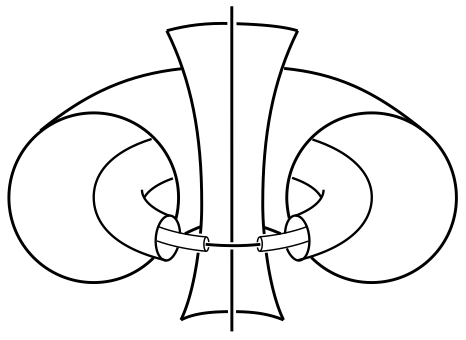
\includegraphics[width=0.5\linewidth]{hopf-bundle}
		\label{fig:hopf-bundle}
	\end{figure}
	The limiting cases $T_0$ and $T_\infty$ correspond to the unit circle in the $xy$-plane and the $z$-axis under the stereographic projection.	Each torus $T_\rho$ is aunion of circle fibers. These fiber circles have slope 1 on the torus, winding around once longitudinally and once meridionally. As $\rho$ goes to $0$ or $\infty$ the fiber circles approach the circles $T_0$ and $T_\infty$, which are also fibers. The figure below shows four tori decomposed into fibers:
	\begin{figure}[H]
		\centering
		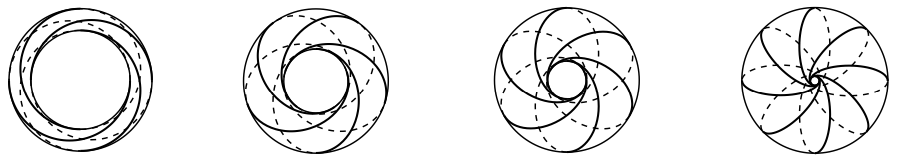
\includegraphics[width=0.9\linewidth]{hopf-bundle2}
		\label{fig:hopf-bundle2}
	\end{figure}
	{\color{persiangreen}How could we visualize the projection onto $S^2$? Could it work to think $S^2=\C\cup\infty$ and just do stereographic projection from 3-space to the plane disregarding one point? What would that even mean hehe}
	
	Replacing the field $\C$ by the quaternions $\H$, the same constructions yield fiber bundles $S^3\to S^{4n+3}\to\H P^{n}$ over quaternionic projective spaces $\H P^n$. Here the fiber $S^3$ is the unit quaternions, and $S^{4n+3}$ is the unit sphere in $\H^{n+1}$. Taking $n=1$ gives a second Hopf bundle $S^3\to S^7\to S^4=\H P^1$.
	
	Another Hopf bundle $S^7\to S^{15}\to S^8$…
\end{example}

\section{model structures}
\begin{defn}[\cite{riehl}]
	A \textbf{\textit{weak factorization system $(\Lc,\Rc)$}} on a category $\Mc$ is comprised o two clases of morphisms $\Lc$ and $\Rc$ so that
	\begin{enumerate}
		\item Every morphism in $\Mc$ may be factored as a morphism in $\Lc$ followed by a morphism in $\Rc$:
		\[\begin{tikzcd}
			\bullet\arrow[rr,"f"]\arrow[rd,"\Lc\ni\ell",swap]&&\bullet\\
			&\bullet\arrow[ru,"r\in\Rc",swap]
		\end{tikzcd}\]
		\item The maps in $\Lc$ have the \textbf{\textit{left lifting property}} with respect to each map in $\Rc$ and equivalently the maps in $\Rc$ have the \textbf{\textit{right lifting property}} with respect to each map in $\Lc$, that is, any commutative square
		\[\begin{tikzcd}
			\bullet\arrow[d,"\Lc\ni\ell",swap]\arrow[r]&\bullet\arrow[d,"r\in\Rc"]\\
			\bullet\arrow[ur,dashed]\arrow[r]&\bullet
		\end{tikzcd}\]
		admits a diagonal filler as indicated making both triangles commute. When this lift is unique, we say the factorization system is \textbf{\textit{orthogonal}}.
		\item The classes $\Lc$ and $\Rc$ are each closed under retracts in the arrow category: given a commutative diagram
		\[\begin{tikzcd}
			\bullet\arrow[r]\arrow[d,"t",swap]\arrow[rr,bend left,no head,shift left=.3]\arrow[rr,bend left,no head,shift right=.3]&\bullet\arrow[r]\arrow[d,"s"]&\bullet\arrow[d,"t"]\\
			\bullet\arrow[r]\arrow[rr,bend right,no head, shift right=.3]\arrow[rr,bend right,no head, shift left=.3]&\bullet\arrow[r]&\bullet
		\end{tikzcd}\]
		if $s$ is in that class then so is its retract $t$.
	\end{enumerate}
\end{defn}

\begin{exercise}[3.1.8 from \cite{riehl}]
Verify that the class of morphisms $\Lc$ characterized by the left lifting property against a fixed class of morphisms $\Rc$ is closed under coproducts, closed under retracts, and contains the isomorphisms.
\end{exercise}

\begin{defn}
	Given a contravariant functor $\Fc:\Cc^{\op}\to\Sets$ there is a corresponding category (\textbf{\textit{of elements of $\Fc$}}) that lies over $\Cc$, that is,
	\[\el\Fc\to\Cc\]
	given by
	
	Objects: pairs $(C,X)$ where $C\in\Obj\Cc$ and $X\in\Fc(X)$.
	
	Morphisms: $f:(C,X)\to(C',C')$ are morphisms $f:C\to C'$ such that $\Fc(f)(X')=X$.
\end{defn}
\begin{remark}
	We can use the Yoneda embedding to view $\Cc$ as a subcategory of $\Psh(\Cc)$,
	\[\Cc\hookrightarrow\Psh(\Cc)\]
	And also $\Fc\in\Psh(\Cc)$. In fact, the element category is just the slice category:
	\[\el\Fc\cong\Cc/\Fc.\]
\end{remark}
\begin{question}
	Given $\Dc\to\Cc$ is it isomorphic to $\el\Fc\to\Cc$?
\end{question}
\begin{defn}
	$G:\Dc\to\Cc$ is a \textbf{\textit{discrete fibration}} if for any $d\in\Dc$ and any $f:C\to G(d)$ there exists a unique lift from $f'$ of $f$ to $f\in\Dc$ such that the target ot $f'$ is is $d$. That is,
	\[\begin{tikzcd}
		\bullet\arrow[d,"G",swap]\arrow[r,"\exists!f'",dashed]&d\arrow[d,"G"]\\
		C\arrow[r,"f",swap]&G(d)
	\end{tikzcd}\]
\end{defn}
\begin{remark}
	Given a discrete fibration we may construct a functor $\Fc:\Cc^{\op}\to\Sets$ simply by defining $\Fc(C)=G^{-1}(C)$ and if $C\to C'$ $\cdots\to d$.
\end{remark}

\iffalse
\begin{remark}[Plan]
	Blakers-Massey excision theorem (relies on technical lema, proof from Tom Dieck's book) $\implies$ Cellular approximation. Also $\implies$ Freudental theorem.
\end{remark}\fi

\begin{defn}[Lecture]
	A \textbf{\textit{model structure}} on a category $\Ac$ is a choice of subcategories $\Wc,\Cc,\Fc$ called \textbf{\textit{weak-equivalences}}, \textbf{\textit{cofibrations}} and \textbf{\textit{fibrations}} with the following properties:
	\begin{enumerate}
		\item[0.] All (finite) small limits an colimits.
		\item \textbf{(2 of 3)} Given $\bullet\overset{f}{\to}\bullet\overset{g}{\to}\bullet$, if either 2 out of 3 among $f,g,f\circ g$ are in $\Wc$ then all of them are.
		\item $(\Cc\cap\Wc,\Fc)$ and $(\Cc,\Fc\cap\Wc)$ are both weak factorization systems.
		$(\Bc,\Dc)$ is a weak factorization system. That is,
		\begin{enumerate}
			\item Any morphism in $\Ac$ can be factored as a morphism in $\Bc$ followed by a morphism in $\Dc$.
			\item Lifts:
			\[\begin{tikzcd}[scale cd=1.2]
				\bullet\arrow["f",d,swap]\arrow[r]&\bullet\arrow[d,"g"]\\
				\bullet\arrow[ur,dashed,"\exists"]\arrow[r]&\bullet
			\end{tikzcd}\]
			\item[(c')] Notice that the aciom of retracts is not necessary. $r'\in\Rc\iff$ it satisfies (b) for all $\ell\in\Lc$.
 		\end{enumerate}
	\end{enumerate}
\end{defn}

\begin{defn}\leavevmode
	\begin{itemize}
		\item $X$ is \textbf{\textit{fibrant}} if $X\twoheadrightarrow\pt$.
		\item $X$ is \textbf{\textit{cofibrant}} if \begin{tikzcd}
			X\arrow[r,tail,two heads]&X
		\end{tikzcd}
		\item $X$ is \textbf{\textit{bifibrant}} if \begin{tikzcd}
			0\arrow[r,tail]&X\arrow[r,two heads]&\pt
		\end{tikzcd}
	\end{itemize}
\end{defn}

\begin{examples}[Two interesting model category structures on $\CGWH$]\leavevmode
\begin{enumerate}
	\item \textbf{\textit{Hurewicz model structure}} (Strom).
	\begin{itemize}
		\item Cofibrations:= Huerwicz cofibrations.
		\item Fibrations:= maps $E\to B$ such that for all spaces $X$ [Photo1].
		\item Weak equivalences:= homotopy equivalences.
	\end{itemize}
	\item \textbf{\textit{Quillen model structure}}. Defined on $\Top$.
	\begin{itemize}
		\item Cofibrations = retracts of relative cell complexes.
		\item Fibrations = Serre Fibrations: \begin{tikzcd}
			D^n\arrow[r]\arrow[d]&E\arrow[d]\\
			D^n\times I\arrow[ur,dashed]\arrow[r]&B
		\end{tikzcd}
		\item Weak equivalences: $f:X\to Y$
	\end{itemize}
	Also, we have
	\begin{itemize}
		\item Fibrant: all of $\Obj\Top$.
		\item Cofibrant: $\exists\{\text{CW complexes}\}$.
	\end{itemize}
\end{enumerate}
\end{examples}
\begin{defn}
	Given a category $\Cc$ and a class of morphisms $W\subset\Mor\Cc$, its \textbf{\textit{localization}} is a category $\Cc[W^{-1}]$ such that there is a functor $\Loc_W\Cc\to\Cc[W^{-1}]$ that sends weak equivalences to isomorphisms. Also, its satisfies the universal property that for every $F:\Cc\to\Dc$ such that $F(X)\subset\Iso$, the following diagram commutes
	\[\begin{tikzcd}
		&\Cc[W^{-1}]\arrow[dr,dashed,"\exists!G"]\\
		\Cc\arrow[ur,swap,"\Loc_W",swap]\arrow[rr,"F"]&&\Dc
	\end{tikzcd}\]
\end{defn}
\begin{thm}
	Let $\Cc$ and $(C,W,F)$ be a model category and $\Cc[W^{-1}]\cong\Ho\Cc$ where the latter is given by
	\begin{itemize}
		\item $\Ob\Ho\Ec=\{\text{fibrant-cofibrant-bifibrant objects of }\Ec\}$.
		\item $\Mor\Ho\Ec=\Mor_{\Ec}(X,Y)/\text{homotopy}$.
	\end{itemize}
\end{thm}
Let's say what homotopy means
\begin{defn}
	Given two maps
	\[\begin{tikzcd}
		X\arrow[r,shift={(0,0.08)},"f"]\arrow[r,shift={(0,-0.08)},swap,"g"]&Y
	\end{tikzcd}\]
	\begin{itemize}
		\item We say $f\underset{\text{left}}{\sim}g$ if for the \textbf{\textit{cylinder}} $\Cyl(X)$ defined by
		\[\begin{tikzcd}
			X\sqcup X\arrow[rr]\arrow[dr,tail,swap,"\text{cofibr.}"]&&X\\
			&\Cyl(X)\arrow[ur,two heads,swap,"\text{trivial fib.}"]
		\end{tikzcd}\]
		we have that
		\[\begin{tikzcd}
			X\sqcup X\arrow[rr,"(f\text{,}g)"]\arrow[dr]&&Y\times Y\\
			&\Cyl(X)\arrow[ur,"\exists H",swap,dashed]
		\end{tikzcd}\]
		\item We say $f\underset{\text{right}}{\sim}g$ if
		\[\begin{tikzcd}
			X\sqcup X\arrow[rr,"(f\text{,}g)"]\arrow[dr,"\exists H",swap,dashed]&&Y\times Y\\
			&\Path(Y)\arrow[ur]
			\end{tikzcd}\]
	\end{itemize}
\end{defn}
\begin{claim}
	Given \begin{tikzcd}
		X\arrow[r,shift={(0,0.08)},"f"]\arrow[r,shift={(0,-0.08)},swap,"g"]&Y
	\end{tikzcd}, if $X$ is cofibrant and $Y$ is fibrant, then $f\underset{\text{left}}{\sim}g\iff f\underset{\text{right}}{\sim}g$ and $\sim$ is an equivalence relation.
\end{claim}


\section{whitehead theorem}

We introduce a large class of spaces, called CW complexes, between which a weak equivalence is necessarily a homotopy equivalence. Thus, for such spaces, the homotopy groups are, in a sense, a complete set of invariants. Moreover, we shall see that every space is weakly equivalent to a CW complex.
\begin{defn}[\cite{may}]\label{defn:CW-complex}\leavevmode
	\begin{enumerate}
		\item A \textbf{\textit{CW complex}} $X$ is a space $X$ which is the union of an expanding sequence of subspaces $X^n$ such that, inductively, $X^0$ is a discrete set of points (called \textbf{\textit{vertices}}) and $X^{n+1}$ is the pushout obtained from $X^n$ by attaching disks $D^{n+1}$ along \textbf{\textit{attaching maps}} $j:S^n\to X^n$. {\color{cyan}Thus $X^{n+1}$ is the quotient space obtained from $X^n\cup(J_{n+1}\times D^{n+1})$ by identifying $(j,x)$ with $j(x)$ for $x\in S^n$, where $J_{n+1}$ is the discrete set of such attaching maps $j$ (see \cref{adjuntion-space})}. Each resulting map $D^{n+1}\to X$ is called a \textbf{\textit{cell}}. The subspace $X^n$ is called the \textbf{\textit{$n$-skeleton}} of $X$.
			\[\begin{tikzcd}
			S^n\arrow[r,"i",hook]\arrow[d,swap,"j"]&D^{n+1}\arrow[d,]\\
			X^n\arrow[r]&X^{n+1}\arrow[ul, phantom, "\ulcorner", very near start]
		\end{tikzcd}\]
	\end{enumerate}
\end{defn}
\begin{lemma}[HELP]
	content...
\end{lemma}
\begin{thm}[Whitehead, \cite{may}]
	If $X$ is a CW complex and $e:Y\to Z$ is an $n$-equivalence, then $e_*:[X,Y]\to[X,Z]$ is a bijection if $\dim X<n$ and surjection if $\dim X=n$.
\end{thm}
\begin{thm}[Whitehead, \cite{may}]\label{thm:W2}
	An $n$-equivalence between CW complexes of dimension less than $n$ is a homotopy equivalence. A weak equivalence between CW complexes is a homotopy equivalence.
\end{thm}
\begin{thm}[Whitehead (4.5), \cite{hatcher-at}]
	If a map $f:X\to Y$ between connected CW complexes induces isomorphisms $f_*:\pi_n(X)\to\pi_n(Y)$ for all $n$, then $f$ is a homotopy equivalence. In case $f$ is the inclusion of a subcomplex $X\hookrightarrow Y$, the conlusion is stronger: $X$ is a deformation retract of $Y$.
\end{thm}
\begin{exercise}[Hatcher 4.1.12]
	Show that an $n$-connected, $n$-dimensional CW complex is contractible.
\end{exercise}
\begin{proof}[Solution]
	Just recall that $n$-connectedness means that $\pi_i(X)=0$ for all $i\leq n$, which means that $X$ is contractible by \cref{thm:W2}.
\end{proof}
\section{lecture notes}
\subsection{14 mar}

\[(X^Y)^Z\cong Z^{Y\times X}\]

\begin{align*}
	g:X'\to X\\\\
	\Hom(X,Y)\mapsto\Hom(X',Y)
\end{align*}

\begin{align*}
	\Hom(A,B)&\cong\Hom(A,B')\text{ natual in }A\implies\\ \Hom(B,B)\cong\Hom(B,B')&\& \Hom(B',B)\cong\Hom(B',B')\\\implies B&\cong B'.
\end{align*}


\begin{itemize}
	\item for $(\impliedby)$ commutativity of the hypotesis gives us commutativiuty of the rightmost square in the diagram below. In fact, the double square diagram below is a rephrasing of the hypothesis.
	
	\item Lemma 2. To build CW complexes
	\item What we did? Prove the bijection between the homotopic sets given an $n$-equivalence.
	\item $\pi_n$ of loop space is the same as $\pi_{n+1}$ of original space.
	\item Then we moved on to homotopic pushouts and pullback. We saw, for instance, that if in a double square diagram each of the squares is a homotopic pushout, then so is the outer square.
	\item We also looked at those exact sequences on cofibers, spaces of homotopy classes, cohomology and (barely) loop spaces. There was a lemma about this.
	\item Next time: cofiber of cofiber is homotopy equivalence, then fibers, fibrations and probably *some name* theorem.
\end{itemize}

\subsection{18 mar}
%Recall some basic definitions:

%\begin{defn}
%	A map $p:E\to B$ has the \textbf{\textit{homotopy lifting property (HLP)}} for the space $X$ if the following holds: for each homotopy $h:W\times I\to B$ and each map $a:X\to E$
%\end{defn}
\begin{lemma}[Yoneda]	
	\[\left\{\text{Natural transformations }\Hom(-,X)\to F\right\}\cong F(X)\]
\end{lemma}
\begin{coro}
	$(\Hom(-,X)\to\Hom(-,Y))\cong\Hom(X,Y)$.
\end{coro}
\begin{coro}
	The correspondence $X\mapsto\Hom(-,X)$ is fully faithful, that is, the correspondence $\Hom(X,X')\to\Hom(\Hom(-,X),\Hom(-,X'))$ is injective and bijective. (The right hand side are natural transformations of functors.)
\end{coro}
\begin{proof}[Solution of exercise 1] The latter correspondence sends isomorphisms to isomorphisms. Since we are given a natural isomorphism in the problem, we conclude $X\cong X'$.
\end{proof}

\begin{lemma}
	Let $E\times_BX$ be the pullback of
	\[\begin{tikzcd}
		&E\arrow[d,two heads]\\
		X\arrow[r,"\simeq"]&B
	\end{tikzcd}\]
	be such that $E\to B$ is an homotopy fibration and $f:X\to B$ is a homotopy equivalence. Let
	\[\begin{tikzcd}
		E\times_BX\to E\arrow[r,dash,"\simeq"]\arrow[d,two heads]&E\arrow[d,two heads]\\
		X\arrow[r,"\simeq"]&B
	\end{tikzcd}\]
	be the pullback. Then $E\times_BX\to E$ is a homotopy equivalence.
\end{lemma}
\begin{proof}
	Let $g:B\to X$ be the homotopy inverse of $f$.
	
	\textbf{(Step 1)} Construct another pullback
	\[\begin{tikzcd}
		E\times_BB\arrow[r]\arrow[d,two heads]&X\times_BE\arrow[r]\arrow[d,two heads]&E\arrow[d,two heads]\\
		B\arrow[r,"g",swap]&X\arrow[r,"f",swap]&B
	\end{tikzcd}\]
	
	\textbf{(Step 2)} Constuct $E\to E\times_BB$.
	
	Consider
	\[\begin{tikzcd}
		E\arrow[rr,"\id"]\arrow[d]&&E\arrow[d,two heads]\\
		E\times I\arrow[r,"f\times \id",swap]\arrow[rru,dashed]&B\times I\arrow[r]&B?
	\end{tikzcd}\]
	And then $E\to E\times_BB\to E\times_BX\to E$ is homotopic to the identity.
	
	Constructing the other homotopic inverse is the hard part.
	
	\[\begin{tikzcd}
		Z\sqcup Z\arrow[d,swap,"f_1\sqcup f_2"]\arrow[r]\arrow[rdd,bend left]&I\times Z\arrow[ld,dashed]\arrow[d]\arrow[dd,bend left]\\
		E\times_BX\arrow[r]\arrow[d]&E\arrow[d]\\
		X\arrow[r,"\simeq"]&B
	\end{tikzcd}\]
\end{proof}
\begin{coro}
	$B\overset{f}{\to}B$ is homotopy equivalence and $E\to B$ is a fibration, in
	\[\begin{tikzcd}
		E\times_BB\arrow[d]\arrow[r]&E\arrow[d]\\
		B\arrow[r,"f",swap]&B
	\end{tikzcd}\]
	$E\times_BB\to E$ is a homotopy equivalence.
\end{coro}

\begin{exercise}
	If $fg$ is an isomorphism and $f$ and $g$ have right inverses, then $f$ and $g$ are isomorphisms.
\end{exercise}

\begin{lemma}
	Let
	\[\begin{tikzcd}
		A\arrow[d,"g",tail]\arrow[r,"f"]&B\arrow[d]\\
		X\arrow[r]&X\cup_AB
	\end{tikzcd}\]
	be a pushout with $A\to X$ a cofibration. Then the canonical map from the double mapping cylinder $M(f,g)\to X\cup_AB$ is a homotopy equivalence.
\end{lemma}
\begin{remark}
	\[\begin{tikzcd}
		A\arrow[d,"g"]\arrow[r,"f"]&B\\
		X
	\end{tikzcd}\qquad \begin{tikzcd}
		A\arrow[d]\arrow[r,hook]&M_f\arrow[d]\\
		X\arrow[r]&X\cup_AM_f\cong M(f,g)
	\end{tikzcd}\]
\end{remark}

\begin{defn}\leavevmode
	\begin{itemize}
		\item The \textbf{\textit{homotopy pullback}} of a diagram
		\[\begin{tikzcd}
			&Y\arrow[d]\\
			X\arrow[r]&Z
		\end{tikzcd}\]
		is
		\[\begin{tikzcd}
			X\times_{\ev_0}Z^I\times_{\ev_1}Y\arrow[d]\arrow[r]&Y\arrow[d]\\
			X\arrow[r]&Z
		\end{tikzcd}\]
		Intuitively, for any $x\in X$ and $y\in Y$ this object has the space of paths connecting $x$ and $y$.
		
		\item The \textbf{\textit{homotopy fiber}} if $f:Y\to Z$ is the pullback of
		\[\begin{tikzcd}
			&Y\arrow[d,"f"]\\
			pt\arrow[r]&Z
		\end{tikzcd}\]
		$F\subset Z^I\times_ZY\to Z$, where $F$ is the space of paths starting at $x$ and ending at the same point $f(y)$.
	\end{itemize}
\end{defn}
\begin{remark}
	The pullback of
	\[\begin{tikzcd}
		&Z^I\times_ZY\arrow[d]\\
		X\arrow[r]&Z
	\end{tikzcd}\]
	is the homotopy pullback of
	\[\begin{tikzcd}
		&Y\arrow[d]\\
		X\arrow[r]&Z
	\end{tikzcd}\]
\end{remark}
\begin{lemma}
	If $X\to Z$ is a fibration then for
	\[\begin{tikzcd}
		&Y\arrow[d]\\
		X\arrow[r,two heads]&Z
	\end{tikzcd}\]
	the map from the pullback to the homotopy pullback is a homotopy equivalence.
\end{lemma}
\begin{proof}
	\[\begin{tikzcd}
		X\times_Z\arrow[r]\arrow[d,"\simeq",dash]&Y\arrow[d,"\simeq"]\\
		X\times_{\ev_0}Z^I\times_{\ev_1}Y\arrow[r,two heads]\arrow[d]&Z^I\times_ZY\arrow[d,two heads]\\
		X\arrow[r]&Z
	\end{tikzcd}\]
\end{proof}

Finally,
\[\begin{tikzcd}
	\hofib f_1\arrow[r]\arrow[d]&\hofib f\arrow[d,two heads]\arrow[r]&*\arrow[d]\\
	*\arrow[r]&X\arrow[r,"f"]&Y
\end{tikzcd}\]
and
\[\begin{tikzcd}
	Z\arrow[dd]\arrow[r]&F(f)\arrow[d]\arrow[dd,bend left,two heads]\\
	&X\times_YY^I\quad\arrow[d]\\
	X\times I\arrow[r]\arrow[uur,dash]&X
\end{tikzcd}\]
and an exact sequence
\[\begin{tikzcd}[column sep=tiny]
	\Omega^2\hofib\arrow[r]&\Omega^2X\arrow[r]&\Omega^2Y\arrow[r]&\Omega\hofib f\arrow[r]&\Omega X\arrow[r]&\Omega Y\arrow[r]&\hofib f\arrow[r]&X\arrow[r,"f"]&Y
\end{tikzcd}\]
\begin{lemma}[Exactness]
	$\forall z$, $[z\hofib f]\to[Z,X]\to[Z,Y]$.
\end{lemma}
and we get the exact sequence
\[\begin{tikzcd}[column sep=tiny]
	\pi_0(\Omega^2X)\arrow[r]&\pi_0(\Omega^2Y)\arrow[r]&\pi_0(\Omega\hofib f)\arrow[r]&\pi_0(\Omega X)\arrow[r]&\pi_0(\Omega Y)\arrow[r]&\pi_0(\hofib f)\arrow[r]&\pi_0(X)\arrow[r]&\pi_0(Y)
\end{tikzcd}\]
and then
\[[S^0,\Omega^2X]=[\Sigma S^0,\Omega X]=[\Sigma^2 S^0,X]=[S^2,X]=\pi_2(X)\]


\subsection{Serre fibration long exact sequence (21 march)}

We've been talking a lot about Hurewickz fibrations. Let's talk about Serre fibrations. Notice that H. fibration $\implies$ S. fibration. What is the most natural example of a Serre fibration?

\begin{prop}[also \cite{hatcher-at} 4.48]
	Let $E$ be a fiber bundle with fiber $F$. Then $f$ is a Serre fibration.
\end{prop}
\begin{proof}
	What sdoes it mean to be a Serre fibration? It means that
	\[\begin{tikzcd}
		I^n\arrow[r]\arrow[d]&E\arrow[d]\\
		I^{n+1}=I^n\times I\arrow[r]\arrow[ur,dashed]&B
	\end{tikzcd}\]
	So if $\Uc$ is a covering of $B$ such that $f^{-1}U\cong U\times F$. By Lebesgue lemma, there is a $\delta>0$ such that for all $x\in I^{n+1}$, the ball $B(x,\delta)$ lies in some $f^{-1}U$ for some $U$.
	
	Then we subdivide $I^{n+1}$ in smaller cubes of the same size with diameter $<\delta$. So, each the image of each cube lies in some $U\in\Uc$.
	
	Then
	\[\begin{tikzcd}
		I^n\arrow[d]\arrow[r]&F\times U\arrow[d,two heads]\\
		I^{n+1}\arrow[r]\arrow[ur,dashed]&U
	\end{tikzcd}\]
	has a lift for every little square because
	\[\begin{tikzcd}
		X\arrow[r]\arrow[d]&U\arrow[d]\\
		X\times I\arrow[r]\arrow[ur,dashed]&pt
	\end{tikzcd}\]
	is always a fibration {\color{orange}(think about this)} and because pullbacks of fibrations are fibrations:
	\[\begin{tikzcd}
		U\times F\arrow[r,two heads]\arrow[d,two heads]&U\arrow[d,two heads]&\\
		F\arrow[r,two heads]&pt
	\end{tikzcd}\].
	Then we may just add up the squares because
	\[\begin{tikzcd}
		D^n\arrow[d]\\
		D^n\times I
	\end{tikzcd}\]
	and we're done.
\end{proof}
\begin{prop}[Sere fibration long exact sequence, see \cref{thm:serre-fibrations-hatcher}]\label{thm:serre-fibrations-lectures}
	Let $g:E\to B$ is a Serre fibration. $e\in E$, $g(e)= b$ and $g^{-1}=F$. Then consider the exact sequence in homotopy of the Serre fibration and the relative homotopy exact sequence. Then there is a long exact sequence (top row):
	\[\begin{tikzcd}
		\cdots\arrow[r]&\pi_n(F)\arrow[r]&\pi_n(E)\arrow[r]&\pi_n(B)\arrow[r]&\pi_{n-1}(F)\arrow[r]&\pi_{n-1}(E)\arrow[r]&\cdots\\
		\cdots\arrow[r]&\pi_n(F)\arrow[r]\arrow[u,"="]&\pi_n(E)\arrow[r]\arrow[u,"="]&\pi_n(E,F)\arrow[r]\arrow[u,"\cong",dashed]&\pi_{n-1}(F)\arrow[r]\arrow[u,"="]&\pi_{n-1}(E)\arrow[r]\arrow[u,"="]&\cdots
	\end{tikzcd}\]
\end{prop}
\begin{example}
	We have shown that $\pi_2(\C P^n)\cong\Z$ using the Hopf fibration $S^1\hookrightarrow S^{2n+1}\to\C P^n$ and the fact that $\pi_k(S^n)=0$ for $k<n$.
\end{example}
\begin{thm}
	Let $X$ be a CW-comples, $A,B\subset X$ subcomplexes, $C=A\cap B\neq\varnothing$, so
	\[\begin{tikzcd}
		C\arrow[r]\arrow[d]&A\arrow[d]\\
		B\arrow[r]&X \arrow[ul, phantom, "\ulcorner", very near start]
	\end{tikzcd}\]
	is a pushout (this happens for inclusions, {\color{orange} check it?}).
	
	If $(A,C)$ is $n$-connected and $(B,C)$ is $m$-connected, then
	\[\pi_i(A,C)\to\pi_i(X,B)\]
	is an isomorphism for $i<m+n$ and sujerctive for $i=m+n$.
\end{thm}

\subsection{blakers-massey (26 march)}
First I show some basic constructions from Tom Dieck (sec. 5.7). Let $f:X\to Y$ be a map. Consider the pullback
\[\begin{tikzcd}
	W(f)\arrow[r]\arrow[d,"(q\text{,}p)",swap]&Y^I\arrow[d,"(\ev_0\text{,}\ev_1)"]\\
	X\times Y\arrow[r,"f\times\id",swap]&Y\times Y
\end{tikzcd}\]
where
\begin{gather*}
	W(f)=\{(x,w)\in X\times Y^I|f(x)=w(0)\},\\
	q(x,w)=x,\quad p(x,w)=w(1).
\end{gather*}
Since $(\ev_0,\ev_1)$ is a fibration, the maps $(q,p)$, $q$ and $p$ are fibrations.

Now suppose $f$ is a pointed map with base points $*$. Then $W(f)\to W'$ is given the base point $(*,k_*)$.

Let $f:A\hookrightarrow X$ be an inclusion.

\begin{defn}
	By $(I^n,\partial I^n)\to (*\times_{\ev_0}X^I\times_{\ev_1}A,\pt)$ is the same as a map $I^n\times I\to X$ that satisfies:
	\begin{itemize}
		\item $I^n\{0\}\cup\partial I^n\times I\to*$.
		\item $I^n\times\{1\}\to A$.
	\end{itemize}
\end{defn}
It is fairly straightforward to show that
\[\begin{tikzcd}
	\cdots\arrow[r]&\Omega A\arrow[r]&\Omega X\arrow[r]&\hofib\arrow[r]&A\arrow[r]&X
\end{tikzcd}\]
\[\begin{tikzcd}
	\pi_0(\nearrow)=&\pi_n(A)\arrow[r]&\pi_n(X)\arrow[r]\arrow[dr]&\pi_{n-1}(\hofib)\arrow[d,"\cong"]\arrow[r]&\pi_{n-1}(A)\arrow[r]&\pi_{n-1}(X)\\
	&&&\pi_n(X,A)\arrow[ur]
\end{tikzcd}\]
\begin{thm}[Blakers-Massey 1]
	Let 
	\[\begin{tikzcd}
		Q\arrow[r,"g"]\arrow[d,swap,"f"]&Y\arrow[d]\\
		X\arrow[r]&P
	\end{tikzcd}\]
	be a homotopy pushout, $g$ is $m$ equivalence, $f$ is $n$-equivalence and $m,n\geq0$. Then $Q\to X\times_P^h$ is $(m+n-1)$-equivalence.
\end{thm}
\begin{thm}[Blakers-Massey 2]
	$P$ is a CW-complex, $X$, $Y$ subcomplexes, $X\cap Y=Q\neq\varnothing$ (\textbf{\textit{strict pushout}})
	\[\begin{tikzcd}
		Q\arrow[r,tail]\arrow[d,tail]&Y\arrow[d,tail]\\
		X\arrow[r,tail]&X\arrow[ul, phantom, "\lrcorner", very near start]
	\end{tikzcd}\]
	Then $\pi_i(Y,\Q)\to\pi_i(P,X)$ is epi for $i=m+n$ and iso for $0\leq i<m+n$.
\end{thm}
\begin{thm}[Blakers-Massey 3]
	$P=X\cup Y$, $X$ and $Y$ are open in $P$, $X\cap Y=Q\neq\varnothing$.
\end{thm}
We proved the third version based on Tom Dieck's proof.
\begin{defn}\leavevmode
	\begin{itemize}
		\item 	A map is a \textbf{\textit{$k$-equivalence}} if the induced map on the $i$th homotopy group is an isomorphism for $i<k$ and an epimorphism for $i=k$.
		\item $K_p(W):=\{x\in W:\text{ at least $p$ coordinates of $x$ are < the same coordinates of the center of }W\}$
	\end{itemize}
\end{defn}
\begin{lemma}
	Let $W$ be a cube in $\R^d$ with $\dim W\leq d$. If for all faces $W'$ of $\partial W$, $f(W')\in A\implies w'\in K_p(W')$, then there is a homotopy $f\simeq g\;\rel\partial W$ such that $g(w)\in A\implies w\in K_p(W)$.
\end{lemma}

\subsection{freudenthal theorem (2 april)}
\begin{defn}
	The appropriate analogue of the Cartesian product in the category of based spaces is the \textbf{\textit{smash product}} $X\wedge Y$ defined by
	\[X\wedge Y=X\times Y/X\vee Y.\]
	Here $X\vee Y$ is viewed as the subspace of $X\times Y$ consisting of those pairs $(x,y)$ such that either $x$ is the basepoint of $X$ or $y$ is the basepoint of $Y$.
\end{defn}
We also have the \textbf{\textit{suspension of pointed spaces}}, which is like usual suspension but also collapsing the distinguished point, which has become an interval:
\[\Sigma X=(I\times X)/(t,x)\sim (0,y)\sim (1,y)\;\forall y\in X.\]


Then we have
\[\Hom_{\CGWH_*}(\Sigma X,\Sigma X)\cong\Hom_{\CGWH_*}(X,\Omega\Sigma X)\]
where $\Sigma X=S^\wedge X$ and $\Omega\Sigma X=\Map(S^1,\Sigma X)$. That is, $S^1\wedge-$ is adjoint to $\Map(S^1,-)$.

So let $X$ be a space. The identity map $\id_{\Sigma X}:\Sigma X\to \Sigma X$ then induces a map $X\to\Omega\Sigma X$.
\begin{thm}[Freudenthal]\label{thm:freudenthal}
	Let $X$ be $\ell$-connected space. Then $X\to\Omega\Sigma X$ is a $(2\ell+1)$-equivalence, that is,
	\[\pi_i(X)\to \pi_{i+1}(\Sigma X),\]
	is a bijection for $i<2\ell+1$ {\color{cyan}and a surjection for $i=2\ell+1$ (\cite{may})}.
\end{thm}
\begin{proof}[Proof 1]
	\[\begin{tikzcd}
	X\arrow[rr,"(\ell+1)\text{-equiv}"]\arrow[rd]\arrow[dd,"(\ell+1)\text{-equiv}",swap]&&*\arrow[dd]\\
	&\Omega \Sigma X \arrow[rd, phantom, "\lrcorner_h", very near start]\arrow[ur]\arrow[ld]\\
	*\arrow[rr]&&\Sigma X\arrow[ul,phantom,"\prescript{h}{}\ulcorner ",very near start]
	\end{tikzcd}\]
\end{proof}
\begin{proof}[Proof 2]
	Consider
	\[\begin{tikzcd}
		X\arrow[r]\arrow[d]&CX\arrow[d]\\
		CX\arrow[r]&\Sigma X
	\end{tikzcd}\]
	Then we use relative homotopy long exact sequence with $(X,CX)$ to get $\pi_i(CX,X)\cong\pi_{i-i}(X)$, which is zero for $0\leq i\leq \ell+1$. Then use relative homotopy exact sequence for the pair $(\Sigma X,CX)$. then we get that $\pi_i(\Sigma X,CX)=\pi_i(\Sigma X)$. And then if you use it for $(\Sigma X, X)$ and 
	
	But it also turns out that $\pi_i(\Sigma X)=\pi_{i-1}(\Omega\Sigma X)$ because
	\begin{align*}
		\pi_n(Z)&=\Hom_{\hTop,*}(S^n,Z)=\Hom(S^1\wedge S^{n-1},Z)=\Hom(S^{n-1},\Omega Z)=\pi_{n-1}(\Omega,Z)
	\end{align*}.
	And then since $CX\hookrightarrow \Sigma X$ we get an arrow $\pi_i(CX,X)\to\pi_i(\Sigma X,CX)$ which is isomorphism for $0\leq i \leq 2\ell +1$ and surjective for $i=2\ell+2$.
	
	So apply Blakers-Massey an ell equalities to get maps fro $\pi_{i-1}(X)\to\pi_{i-1}(\Omega\Sigma X)$ for $i$ as desired.
\end{proof}
\begin{coro}
	If $X$ is $\ell$-connected, then $\Sigma X$ is $(\ell+1)$-connected for $\ell\geq0$.
\end{coro}
\[\begin{matrix}
	\text{space}&&S^0&\Sigma S^0=S^1&\Sigma^2S^0=S^2&\Sigma^3S^0=S^3&\cdots&\Sigma^nS^0=S^n\\
	\text{conectedness}&&-1&0&1&2&\cdots&(n-1)
\end{matrix}\]
\begin{coro}
	$S^n$ is $(n-1)$-connected.
\end{coro}
Back to Hopf fibration:
\[S^1\hookrightarrow S^3\to S^2\]
we get
\[0=\pi_2(S^3)\to\pi_2(S^2)\overset{\cong}{\to}\pi_1(S^1)\to\pi_1(S^3)=0,\]
so
\[\Z=\pi_2(S^2).\]
Now consider a map $S^n\to S^n$. We get a map $CS^n\to CS^n$ (in general, for $f:X\to Y$ we have $(t,x)\mapsto(t,f(x))$ in the cones). We also have $CS^n\to CS^n/S^n=S^{n+1}$.

Now if we take $\id:S^n\to S^n$ we shall get $\id:S^{n+1}\to S^{n+1}$. Think about this like $\pi_1(S^1)\to\pi_2(S^2)$. Now from Freudenthal we get $\pi_{i-1}(X)\to\pi_i(\Sigma X)$ is surjective because $i=0$. From Hopf fibration we have $\pi_2(S^2)=\Z$. So we have a surjective map $\Z\to\Z$. So it's an isomorphism and we conclude that $\id_{S^2}$ is a generator of $\pi_2(S^2)$.

\begin{coro}
	Since $S^n$ is $(n-1)$-connected, we have
	\[\pi_i(S^n)\to\pi_{i+1}(S^{n+1})\]
	is isomorphism for $i\leq 2(n-1)=2n-1$ and epimorphism form $i=2n-1$. (We just shift the indices of \cref{thm:freudenthal} by one.)
\end{coro}
\begin{coro}
	$\pi_n(S^n)=\Z$ with $\id_{S^n}$ as generator.
\end{coro}
\begin{coro}
	$\pi_{n+k}(S^n)\to\pi_{n+k+1}(S^{n+1})$ is isomorphism for $k\leq n-1$ and epimorphism for $k=n-1$.
\end{coro}
So for example
\[\pi_4(S^3)=\pi_5(S^4)=\pi_6(S^5).\]
And in fact they are $\Z/2$. This is what are called the \textbf{\textit{$k$th stable homotopy groups of a sphere}}. And more in general, we take any space and apply $\Omega\Sigma$ enough times, and the homotopy will start to stabilize.

Or for example from
\[S^1\hookrightarrow S^3\to S^2\]
we get
\[0=\pi_i(S^1)\to \pi_i(S^3)\overset{\cong}{\to}\pi_i(S^2)\to\pi_{i-1}(S^2)=0\]
So $\pi_3(S^2)\cong\Z$ in case you were wondering.
\begin{claim}[Serre]
	$\pi_{4n-1}(S^{2n})\cong\Z\oplus$finite abelian. And $\pi_i(S^k)$ is finite abelian in all other cases.
\end{claim}

\subsection{another application of Blakers-Massey (2 april)}
Glue a disk to a space and what happens to homotopy groups?
\[\begin{tikzcd}
	S^{n-1}\arrow[r,"(n-1)\text{-equiv}"]\arrow[d,"0\text{-equiv}",swap]&D^n\arrow[d]\\
	X\arrow[r]&X\cup D^n\arrow[ul, phantom, "\ulcorner", very near start]
\end{tikzcd}\]
Assume $X$ is connected. We get a map from the vertical arrows
\[\begin{tikzcd}
	\pi_i(D^n,S^{n-1})\arrow[r]&\pi_i(X\cup D^n,X)
\end{tikzcd}\]
which is $(n-1)$-equivalence by Blakers-Massey. So, by attaching $\sqcup D^n$ we can kill $\pi_{n-1}(X)$, that is, $X\cup(\sqcup D^n)$ has trivial $\pi_{n-1}$.

Now notice that

%since $S^{n-1}\to D^n$ is an $(n-1)$-equivalence, which is the case since
\[\begin{tikzcd}
	0=\pi_i(D^n)\arrow[r]&\pi_i(D^n,S^{n-1})\arrow[r,"\cong"]&\pi_{i-1}(S^{n-1})\arrow[r]&\pi_{i-1}(D^n)=0
\end{tikzcd}\]
that is, $\pi_i(D^n,S^{n-1})=0$ for $i\leq n-1$. This implies that $\pi_i(X\cup D^n,X)=0$ for $i\leq n-1$.

Also by homotopy long exact sequence,
\[\pi_{n-1}(X)\to \pi_i(X\cup D^n)\text{ is sujrective}\]
\[\pi_i(X)\to \pi_{i}(X\cup D^n)\text{ is isomorphism for }i\leq n-2.\]
So what we have thus far is
\[\begin{tikzcd}
	\pi_n(X\cup D^n)\arrow[r]&\pi_{n-1}(X)\arrow[r]&\pi_{n-1}(X\cup D^n)\arrow[r]&0=\pi_{n-1}(X\cup D^n)
\end{tikzcd}\]
Notice that $\pi_n(X\cup D^n,X)$ is not ingeneral cyclic (counterexample $S^1\cup D^2$ taking unieversal cover which is real line with spheres on integers, homotopy equivalent to $\bigvee_\Z S^2$ which is not finitely generated).

\begin{quote}
	{\color{red} So basically attaching a disk via $f$ will kill $[f]$ inside $\pi_n(X)$ this is called \textbf{\textit{killing}} an element of the homotopy group.}
\end{quote}

\begin{prop}
	For any CW-complex $X$, $X^\ell\to X$ is an $\ell$-equivalence.
\end{prop}
\begin{remark}
	We have used that for $A\hookrightarrow X$ from long exact sequence of relative homotopy groups we get $\pi_n(X,A)=0$.
\end{remark}
\begin{coro}
	Let $i\leq \ell$ and $g: D^i\to X$, $g:\partial D^i\to X^\ell$. Then there is a homotopy $\rel\partial D^i$ to a map with $\img\subset X^\ell$.
\end{coro}
\begin{thm}[Cellular approximation theorem]
	Let $X$ and $Y$ be CW-complexes and $\xi:Y\to X$ be any map. Then $\xi$ is homotopic to a \textbf{\textit{cellular map}}, that is, a map $\psi:Y\to X$, such that for all $\ell$, $\psi Y^0\subset X^\ell$.
\end{thm}

We also have
\begin{prop}
	Let $n\geq 2$. Then 
	\[\pi_n\left(\bigvee_{k\in I}S^n\right)=\bigoplus_{k\in I}\i_n(S^n)=\bigoplus_{k\in I}\Z=Z^{\oplus I}\]
\end{prop}
\begin{prop}
	First notice that for finite $I$,
	\[X^n=X^{n+1}=\bigvee_{k\in I}S^n\]
	by looking carefully. Then
	\[\pi_n(X,X^{n+1})=0=\pi_{n+1}(X,X^{n+1})\]
	so
	\[\bigoplus_{k\in I}\Z=\prod_{k\in I}\pi_n(S^n)=\pi_n(X)=\pi_n(X^{n+1})=\pi_n(X^n)=\pi_n\left(\bigvee_{k\in I}S^n\right)\]
	and for the infinite case it also works, using finite compactness of the CW complex.
\end{prop}


\subsection{postnikov tower and CW-approximation, 9 abril}
\begin{itemize}
	\item Let $X$ be a space. Then there is a CW-complex $Y$ and a weak homotopy equivalence from $Y\to X$.
	\item Let $A\to X$ be a map of spaces. Then it can be factored as $A\to Y\to X$ where $A\hookrightarrow Y$ is a relative CW-complex, and $Y\to X$ is a weak homotopy equivalence.

\begin{remark}
	Notice that the second item is the first one with $A=\varnothing$. Then, the second case is a Serre cofibration since it is a construction involving the cofibration $S^{n-1}\hookrightarrow D^n$ (this is a cofibration by definition).
\end{remark}
\item Let $A$ be a space. Then there is a space $\tau_{\leq n}A$ such that $A\hookrightarrow\tau_{\leq n}A$; $\tau_{\leq n}A$ is obtained by adding cells of $\dim\geq n+2$. $A\hookrightarrow\tau_{n\leq n}A$ is $(n+1)$-equivalence and
\[\pi_k(\tau_{\leq n}A)=0\qquad k>n.\]
Moreover, $A\to \tau_{\leq n}A$ is unique among morphisms in $\Ho(CGWH)$ from $A$ into spaces with $\pi_k=0$ for $k>n$.

This is called a \textbf{\textit{Postnikow tower}} and it looks like this:
\[\begin{tikzcd}
	&\cdots\arrow[d]\\
	&\tau_{\leq 2}A\arrow[d]\\
	&\tau_{\leq 1}A\arrow[d]\\
	A\arrow[uur]\arrow[ur]\arrow[r]&\tau_{\leq 0}A
\end{tikzcd}\]
The idea is that $\tau_{\leq n}A$ is obtained from $A$ by killing elements of dimension greater than $n$, that is, by \begin{itemize}
	\item attaching $n+2$ cells that kill all $\pi_{n+1}(A)$,
	\item attaching $n+3$ cells that kill all $\pi_{n+2}(A)$,
	\item attaching $n+3$ …
	\item attaching $n+n$ …
\end{itemize}
So consider the space $X$ that is obtained from $A$ after attaching cells of dimension $\geq n+2$, so we have a map $A\to X$. Consider also a space $Y$ with $\pi_k(Y)=0$ for $k>n$. Then for any map $A\to Y$ there is a map $X\to Y$ that extends $A\to Y$. This accounts for a bijection 
\[[X,Y]\cong[A,Y].\]
In class we struggled a bit to prove surjectivity, finally using an argument related to the pair $(X\times I,X\times\partial I\cup A\times I)$.

\begin{quote}
	{\color{red}The point is that the spaces in the Postnikov tower are like the original space but with trivial homotopy groups for $k\geq n$.}
\end{quote}
\begin{question}
	What is the limit of the Posnikov tower?
	\[\begin{tikzcd}
		&\lim\\
		&\cdots\arrow[d]\\
		&\tau_{\leq 2}A\arrow[d]\\
		&\tau_{\leq 1}A\arrow[d]\\
		A\arrow[uur]\arrow[uuuur]\arrow[ur]\arrow[r]&\tau_{\leq 0}A
	\end{tikzcd}\]
\end{question}

\item Let $A\to X$ be a map (of CW-complexes (or spaces?)). Then
\[\begin{tikzcd}
	&\cdots\arrow[d]\\
	&Y_2\arrow[ddr,bend left]\arrow[d]\\
	&Y_1\arrow[rd]\arrow[d]\\
	A\arrow[uur,bend left]\arrow[ur]\arrow[r]\arrow[rr,bend right]&Y_0\arrow[r]&X
\end{tikzcd}\]
{\color{red}Proof pending}

\item We also have the \textbf{\textit{Whitehead tower}}, obtained from the homotopy fiber
\[\begin{tikzcd}
	\hofib f_n\arrow[r]&A\arrow[r,"f_n"]&\tau_{\leq n-1}A
\end{tikzcd}\]
which yields
\[\begin{tikzcd}[column sep=small]
	\cdots\arrow[r]&\pi_{k+1}(A)\arrow[r,"\cong"]&\pi_{k+1}(\tau_{\leq n}A)\arrow[r]&\pi_k(\hofib)\arrow[r]&\pi_k(A)\arrow[r]&\pi_k(\tau_{\leq n}A)\arrow[r]&\cdots
\end{tikzcd}\]
so
\[\begin{tabular}{|L|L|L|}
	\hline 
	k\leq n-1&k=n&k\geq n+1\\\hline
	\pi_k(\hofib f_n)=0&\pi_n(\hofib f_n)=0&\pi_k(A)=\pi_k(\hofib f_n)\\\hline
\end{tabular}\]

\item Now there's a natural way to construct the following diagram:
\[\begin{tikzcd}
	A\arrow[r]\arrow[rr,bend right]&\tau_{\leq n}A\arrow[r,]&\tau_{\leq n-1}A
\end{tikzcd}\]
which yields the bundle
\[\begin{tikzcd}
	\hofib\arrow[r]&\tau_{\leq n}A\arrow[r,]&\tau_{\leq n-1}A
\end{tikzcd}\]
and in this case we get
\[\begin{tabular}{|L|L|}
	\hline k\neq n&k=n\\\hline
	\pi_k(\hofib)=0&\pi_n(\hofib)=\pi_n(A)\\\hline
\end{tabular}\]
and this is what we call a \textbf{\textit{$\K(\pi,n)$-space}} (all homotopy groups are trivial but the $n$th.)
\end{itemize}

\subsection{11 apr}
\begin{thm}[Uniqueness of CW-approximations]
	Recall that a CW-approximation of $X$ is a map $f:Z\to X$ and a CW-complex $Z$ that is a weak homotopy equivalence (induces isomorphisms in all homotopy groups).
	
	We have that
	\[\begin{tikzcd}
		Y_1\arrow[dr,"\text{CW ap.}"]\\
		&X\\
		Y_2\arrow[uu,dashed,"\exists!"]\arrow[ur,"\text{CW ap.}"]
	\end{tikzcd}\]
	up to homotopy equivalences
\end{thm}
\begin{lemma}[Compression]
	If the relative homotopy groups of a pair $(Y,B)$ is zero for $n=\dim e$ for every cell $e\in X\backslash A$ then any map $(X,A)\to(Y,B)$ is homotopic $\rel A$ to $(X,A)\to (B,B)$ {\color{persiangreen}(so intuitively we can collapse $Y$)}.
\end{lemma}
\begin{proof}
	With fibrations (photo)
\end{proof}
\begin{prop}
	Let $f:X\to Y$ be an $n$-equivalence (in \cite{hatcher-at} stated as weak equivalence but argument is the same). Then $f$ induces an \textit{\textbf{$n$-equivalence in homology}} $H_i(X,\Z)\to H_i(Y,\Z)$ (an isomorphism for $i<n$ and surjection for $i=n$).
\end{prop}
\begin{proof}
	photo
\end{proof}
\begin{coro}
	If $f:X\to Y$ is a weak equivalence, then $f$ induces an isomorphism in $H_*(-,G)$ and $H^*(-,G)$.
\end{coro}
\begin{proof}
	Universal coefficients.
\end{proof}

\begin{defn}
	Let $\pi$ be an abelian group. Take 
	\[\begin{tikzcd}
		F_1\arrow[r]& F_0\arrow[r]& \pi
	\end{tikzcd}\] 
	a \textbf{\textit{free resolution}}, i.e. $F_1=Z^{\oplus J}$ and $F_0=Z^{\oplus I}$ are free abelian groups and $\pi=F_0/F_1$. Let's take the corresponding maps
	\[\begin{tikzcd}[row sep=tiny]
		\bigvee_{j\in S}S^n\arrow[r]&\bigvee_{i\in I}S^n\arrow[r]&\hocofib f\\
		x_j\arrow[r,maps to]&\sum a_iy_i
	\end{tikzcd}\]
	where $a_i$ is the degree of $S^n\to S^n$
	Recall that the homotopy cofiber $\hocofib f$ is the mapping cone of $f$. It is the \textbf{\textit{cone of pointed spaces}}.
\end{defn}
	What do we get in homology? Exactly the sequence of free groups above. So, $H_n(\hocofib f)=\pi$. What do we get in homotopy? {\color{red}Might be $\pi$ as well}. Let's prove something stronger:
	
\begin{thm}
	Let $Y$ be such that $\pi_i(Y)=0$ for $i>n$ and $\pi_0(Y)=0$. Then
	\[[\hocofib f,Y]\to\Hom(\pi_n(\hocofib f),\pi_n(Y))\]
	is a bijection.
\end{thm}
\begin{proof}
	Photo
\end{proof}
\begin{thm}
	Take $\tau_{\leq n}(\hofib f)$ which is a $\K(\pi,n)$ space with cells in $\dim\geq n$, obtained from $\hofib f$ by attaching cells of $\dim\geq n+2$. Then
	\[[\hocofib f,y]\cong[\tau_{\leq n}(\hocofib f), Y]=\Hom(\pi,\pi_n(Y)).\]
	If $\pi_n(Y)=\pi$, then there is a weak equivalence
	\[\tau_{\leq n}(\hocofib f)\to Y.\]
\end{thm}


\begin{defn}
	Let $\Cc$ be a category. Then $\Psh(\Cc)$ is the category of \textbf{\textit{presheaves}} of $\Cc$ i.e. the category of functors $\Cc^{\op}\to\Sets$ and natural transformations. For any object $A$ in $\Cc$ there is a presheaf $\Hom_{\Cc}(-,A)$. A presheaf $\Fc$ that is isomorphic to $\Hom_\Cc(-,A)$ for some $A$ is called \textbf{\textit{representable}}.
\end{defn}
	
For example, $\Hom_{\CW}(X,\K(\pi,n))\cong H^n(X,\pi)$, that is, $H^n$ is representable.
\begin{lemma}[Yoneda]
	Let $G$ be a presheaf, $A$ be an object in $\Cc$. Then
	\[\Nat(\Hom(-,A),G)\cong G(A)\]
	naturally in $A$.
\end{lemma}
\clearpage
%		\arrow[ul, phantom, "\lrcorner", very near start]
%		\arrow[ul, phantom, "\ulcorner", very near start]
\addcontentsline{toc}{section}{References}
\printbibliography
\end{document}